\def\languageisfrench{}
\documentclass[a4paper,8pt]{extarticle} % extarticle allows to use font size of 8pt.

\usepackage[a4paper, top=1.6cm, bottom=2cm, left=1.6cm, right=1.6cm]{geometry} % Marge reduction.

%% Language specific package
\usepackage[french]{babel}
\frenchbsetup{StandardLists=true} % Necessary to use enumitem with babel/french.

%% Font and typing packages
\usepackage{fontspec}
\setmainfont[
	Ligatures=TeX,
	ItalicFont={Dancing Script},
	BoldItalicFont={Dancing Script}
	]{PT Serif} % default is Latin Modern
\newfontfamily\antiquefont[Ligatures=TeX]{Caslon Antique} % fancy font
\usepackage{microtype}			% Greatly improves general appearance of the text.
\usepackage{SIunits}			% Unit appearance.
\usepackage{ulem}				% To cross words out. Use \sout{}.

%% Array utilities
\usepackage{array}				% Additionnal options for arrays.
\usepackage{colortbl}			% Additionnal options for coloring arrays.
\usepackage{multirow}
\usepackage[table]{xcolor}		% Auto alternate grey-white rows.

%% List utilities
\usepackage[inline]{enumitem}   % Display inline lists.
\usepackage{etoolbox}           % General utility. Good for lists for instance.
\usepackage{xparse}             % List utilities.

%% Page utilities
\usepackage{multicol}			% Allows to divide a part of the page in multiple columns.
\usepackage{fancyhdr}		% For custom headers and foot texts
\pagestyle{fancy}
	
%% Others
\usepackage{xstring}            % String parsing, cutting, etc.
\usepackage[hidelinks, bookmarks=false, pdfdisplaydoctitle=true, pdfstartview=FitH, pdfpagelabels=false]{hyperref} % Links in PDF.

\makeatletter

%%% Language specific stuff


\newcommand{\translationteam}{\item \og AEnoriel \fg \item \og Anglachel \fg \item \og Astadriel \fg \item \og Batcat \fg \item \og Bigfish \fg \item \og Eru \fg  \item \og Gandarin \fg \item \og Groumbahk \fg \item \og Iluvatar \fg \item \og Mammstein \fg \item \og Shlagrabak \fg \item et beaucoup d'autres...}

\hypersetup{
	pdfauthor={Équipe de traduction française de T9A},
	pdfsubject={Règles pour le jeu Batailles Fantastiques : Le 9\ieme{} Âge},
}

%%% Commands %%%

\ifdef{\isitanAB}{

\newcommand{\addtosortedlist}[1]{%
	\protected@edef\textarg{#1}%
	\protected@edef\textwithoutspaces{\expandafter\removespaces\expandafter{\textarg}}%
	\substitute\textwithoutspaces{É}{E}% Most used special characters of the language, and equivalent for alphabetical ordering
	\substitute\textwithoutspaces{È}{E}%
	\substitute\textwithoutspaces{Ê}{E}%
	\substitute\textwithoutspaces{é}{e}%
	\substitute\textwithoutspaces{è}{e}%
	\substitute\textwithoutspaces{ê}{e}%
	\substitute\textwithoutspaces{À}{A}%
	\substitute\textwithoutspaces{à}{a}%
	\substitute\textwithoutspaces{ù}{u}%
	\expandafter\sortitem\expandafter[\textwithoutspaces]{#1}%
}%

\newcommand{\pts}[1]{% First step is to remove spaces if there are some
	\def\numberwithoutspaces{\expandafter\removespaces\expandafter{#1}}%
	% Next step is getting rid of formatting if there are any (bold, color, ...)
	\pdfstringdef\cleannumber{\numberwithoutspaces}%
	% Now we can try if it is 1 or not
	\expandafter\ifstrequal\expandafter{\cleannumber}{1}{#1~\labels@point}{%
	\expandafter\ifstrequal\expandafter{\cleannumber}{0.5}{0,5~\labels@point}{%
	\expandafter\ifstrequal\expandafter{\cleannumber}{1.5}{1,5~\labels@point}{%
	#1~\labels@points}}}%
}

}{}

% Dark gods
\newcommand{\dchange}{Changement}
\newcommand{\dlust}{Luxure}
\newcommand{\pestilence}{Pestilence}
\newcommand{\wrath}{Courroux}
\newcommand{\truechaos}{Chaos Primordial}


% Nothing to edit here

\ifdef{\isitanAB}{

\newcommand{\alliancepts}[1]{
\ifsubstring{#1}{\free}{%
		\free{}%
	}{%
	\ifsubstring{#1}{\permodel}{%
		\splitatinf{#1}\myoption\myvalue%
		\pts{\myvalue}\permodel{}%
	}{%
	\pts{#1}
	}}
}

% You might wanna change the order of the gods - advanced user
\newcommand{\allianceoptions}[1]{%
	\defallianceoptions{#1}%
	\unitentryformat{\labels@allianceoptions\spacebeforecolon{}:}\newline
	\expandafter\ifblank\expandafter{\allianceoptions@introsentence}{}{\noindent\allianceoptions@introsentence{}\spacebeforecolon{}:}
	
	\expandafter\ifblank\expandafter{\allianceoptions@wrath}{
		\setlength{\columnseprule}{0.5pt}
		\renewcommand{\columnseprulecolor}{\color{black!30}}
		\vspace*{-0.2cm}\begin{multicols}{3}\raggedcolumns
		
			\begin{center}
			\noindent\dchange{}
			
			\noindent\alliancepts{\allianceoptions@change}
			\vspace*{-0.3cm}
			\end{center}
		
		\columnbreak
		
			\begin{center}
			\noindent\dlust{}
			
			\noindent\alliancepts{\allianceoptions@lust}
			\vspace*{-0.3cm}
			\end{center}
		
		\columnbreak

			\begin{center}
			\noindent\pestilence{}
			
			\noindent\alliancepts{\allianceoptions@pestilence}
			\vspace*{-0.3cm}
			\end{center}
			
		\end{multicols}
		\setlength{\columnseprule}{0pt}	
	}{
		\setlength{\columnseprule}{0.5pt}
		\renewcommand{\columnseprulecolor}{\color{black!30}}
		\vspace*{-0.2cm}\begin{multicols}{4}\raggedcolumns
		
			\begin{center}
			\noindent\dchange{}
			
			\noindent\alliancepts{\allianceoptions@change}
			\vspace*{-0.3cm}
			\end{center}
		
		\columnbreak

			\begin{center}
			\noindent\wrath{}
			
			\noindent\alliancepts{\allianceoptions@wrath}
			\vspace*{-0.3cm}
			\end{center}
		
		\columnbreak
		
			\begin{center}
			\noindent\dlust{}
			
			\noindent\alliancepts{\allianceoptions@lust}
			\vspace*{-0.3cm}
			\end{center}
		
		\columnbreak

			\begin{center}
			\noindent\pestilence{}
			
			\noindent\alliancepts{\allianceoptions@pestilence}
			\vspace*{-0.3cm}
			\end{center}
			
		\end{multicols}
		\setlength{\columnseprule}{0pt}
	}
}

}{}


%%% Labels %%%

% Profile

\newcommand{\labels@M}{M}
\newcommand{\labels@WS}{CC}
\newcommand{\labels@BS}{CT}
\newcommand{\labels@S}{F}
\newcommand{\labels@T}{E}
\newcommand{\labels@W}{PV}
\newcommand{\labels@I}{I}
\newcommand{\labels@A}{A}
\newcommand{\labels@Ld}{Cd}
\newcommand{\labels@Invocation}{Invocation} % For Vampire Covenant profiles
\newcommand{\labels@roundbase}{rond} % printed after XX mm for round bases

\newcommand{\Strength}{Force}

% Technical

\newcommand{\labels@range}{Portée}
\newcommand{\labels@point}{pt}
\newcommand{\labels@points}{pts}
\newcommand{\labels@only}{uniquement}
\newcommand{\labels@magic}{Magie}
\newcommand{\labels@pathsused}{Génère ses sorts dans la Discipline}
\newcommand{\labels@model}{figurine}
\newcommand{\labels@models}{figurines}
\newcommand{\labels@Singlemodel}{Figurine \textbf{seule}}

% Unit entry labels

\newcommand{\labels@basesize}{Socle}
\newcommand{\labels@trooptype}{Type de troupe}
\newcommand{\labels@specialrules}{Règles Spéciales}
\newcommand{\labels@alignment}{Allégeance}
\newcommand{\labels@alliance}{Allégeance}
\newcommand{\labels@allianceoptions}{Options d'Allégeance}
\newcommand{\labels@greenhiderace}{Race de Peaux Vertes}
\newcommand{\labels@equipment}{Équipement}
\newcommand{\labels@weapons}{Armes}
\newcommand{\labels@armour}{Armure}
\newcommand{\labels@options}{Options}
\newcommand{\labels@commandgroup}{État-Major}
\newcommand{\labels@charactermounts}{Montures de Personnages}
\newcommand{\labels@mounts}{Montures}
\newcommand{\labels@mount}{Monture}
\newcommand{\labels@specialequipment}{Équipement Spécial}

% Command groups

\newcommand{\labels@champion}{Champion}
\newcommand{\labels@standardbearer}{Porte-Étendard}
\newcommand{\labels@musician}{Musicien}
\newcommand{\labels@singlebannerallowance}{Une seule unité de ce type peut prendre une Bannière Magique}
\newcommand{\labels@condsinglebannerallowance}{Une seule unité de ce type peut prendre une Bannière Magique si}
\newcommand{\labels@bannerallowance}{Bannière Magique}
\newcommand{\labels@veteranstandardbearer}{Peut devenir Porte-Étendard Vétéran}
\newcommand{\labels@championallowance}{Arme Magique}

% Titles

\newcommand{\labels@armylist}{Liste des Troupes}
\newcommand{\labels@lords}{Seigneurs}
\newcommand{\labels@heroes}{Héros}
\newcommand{\labels@coreunits}{Unités de Base}
\newcommand{\labels@specialunits}{Unités Spéciales}
\newcommand{\labels@rareunits}{Unités Rares}
\newcommand{\labels@armywiderules}{Règles Communes de l'Armée}
\newcommand{\labels@armyspecialrules}{Règles Spéciales de l'Armée}
\newcommand{\labels@armoury}{Armurerie}
\newcommand{\labels@magicalitems}{Objets Magiques}
\newcommand{\labels@magicalweapons}{Armes Magiques}
\newcommand{\labels@magicalarmour}{Armures Magiques}
\newcommand{\labels@talismans}{Talismans}
\newcommand{\labels@enchanteditems}{Objets Enchantés}
\newcommand{\labels@arcaneitems}{Objets Cabalistiques}
\newcommand{\labels@magicalbanners}{Bannières Magiques}
\newcommand{\labels@quickrefsheet}{Fiche de Référence}
\newcommand{\labels@changelog}{Change Log}

\newcommand{\labels@lordsInitial}{S}
\newcommand{\labels@heroesInitial}{H}
\newcommand{\labels@coreunitsInitial}{B}
\newcommand{\labels@specialunitsInitial}{S}
\newcommand{\labels@rareunitsInitial}{R}
\newcommand{\labels@mountsInitial}{M}


% Titlepage

\newcommand{\labels@fantasybattles}{Batailles Fantastiques}
\newcommand{\labels@NinthAge}{Le 9\ieme{} Âge}
\newcommand{\labels@armyrules}{Règles de l'Armée}
\newcommand{\labels@frontpagecredits}{%
\labels@fantasybattles{} : \labels@NinthAge{} est un jeu créé et entretenu par la communauté qui met en scène des affrontements de figurines.\newline
Toutes les règles sont disponibles gratuitement sur le site suivant. Vos retours et suggestions sont les bienvenus : \url{http://www.the-ninth-age.com/}
}
\newcommand{\labels@license}{Copyright Creative Commons license : \url{the-ninth-age.com/license.html}}
\newcommand{\labels@tableofcontents}{Sommaire}
\newcommand{\labels@introduction}{%
\begin{center}\noindent{\Largerfontsize\textbf{Note des traducteurs}}\end{center}
\vspace{0.5cm}

Nous souhaitons remercier chaleureusement l'équipe à l'initiative du 9\ieme{} Âge pour leur motivation et leur travail continu pour faire vivre notre passion. Nous espérons que ce jeu saura développer les qualités pour plaire au plus grand nombre et réunir les joueurs, amateurs comme habitués des tournois, autour de règles amusantes et équilibrées, pour finalement s'imposer comme un standard du jeu de figurines. Une grande ambition qui ne pourra s'accomplir que \textbf{grâce à vous}, la communauté, via des retours constructifs, afin de modeler le jeu selon nos désirs. N'étant \textbf{en aucun cas à but lucratif}, le 9\ieme{} Âge part avec un avantage considérable. Les règles des éventuelles nouvelles sorties ne sont pas dictées par le besoin de vendre ces nouveautés. Vous pouvez choisir et acheter vos figurines où bon vous semble, il n'y a pas un unique revendeur toléré. Enfin, vous pouvez être assurés que tant que le 9\ieme{} Âge sera joué, vous disposerez d'un \textbf{support continu et régulier}, celui-ci étant offert par la communauté.

Concernant la traduction en elle-même, nous avons fait de notre mieux pour vous offrir une version de qualité, dont nous espérons qu'elle surpasse celle de la version originale ! Si vous constatez des coquilles, des erreurs, merci de nous les signaler en nous contactant sur le forum du 9\ieme{} Âge, dans le \textbf{sous-forum français} (\url{http://www.the-ninth-age.com/index.php?board/117-french/}). Vous y trouverez aussi les dernières mises à jour. \textbf{En cas de conflit d'interprétation avec la version originale, la version originale fait référence}.

\vspace{0.5cm}
Que ce jeu vous apporte d'innombrables heures de plaisir partagé !

\vspace{1cm}

\ifdef{\translationteam}{
	\begin{multicols}{3}
	\begin{itemize}
		\translationteam
	\end{itemize}
	\end{multicols}
}{}
}
\newcommand{\labels@rulechanges}{% blank ATM
}
\newcommand{\labels@latexcredit}{Document réalisé à l'aide de \LaTeX .}


%%% Technical commands

\newcommand{\only}[1]{(#1 uniquement)}
\newcommand{\free}{gratuit}
\newcommand{\upto}{jusqu'à}
\newcommand{\Upto}{Jusqu'à}
\newcommand{\unlimited}{pas de limite}
\newcommand{\permodel}{/fig.}
\newcommand{\listlastchoice}{ ou}
\newcommand{\notif}[1]{(pas #1)}
\newcommand{\wordand}{et}
\newcommand{\wordwith}{avec}
\newcommand{\ifNmodelsorless}[1]{(#1 figurines ou moins)}
\newcommand{\unitwith}{unité avec}
\newcommand{\From}{De} % From ... to ... models
\newcommand{\wordto}{à}
\newcommand{\wordAll}{Tous}
\newcommand{\spacebeforecolon}{ } % French put a space before colons
\newcommand{\minprice}{Coût min. :}
\newcommand{\mincostfor}{Coût min. pour}
\newcommand{\maxunitsize}{Taille max.}
\newcommand{\additionalfigscost}{Les figurines additionnelles coûtent}


%%% Special rules %%%

\newcommand{\ambush}{Embuscade}
\newcommand{\armourpiercing}[1]{Perforant\ifblank{#1}{}{ (#1)}}
\newcommand{\bodyguard}[1]{Garde du Corps\ifblank{#1}{}{ (#1)}}
\newcommand{\breathweapon}[1]{Attaque de Souffle\ifblank{#1}{}{ (#1)}}
\newcommand{\channel}{Canalisation}
\newcommand{\crushattack}{Attaque Écrasante}
\newcommand{\daemonicinstability}{Instabilité Démoniaque}
\newcommand{\devastatingcharge}{Charge Dévastatrice}
\newcommand{\distracting}{Distrayant}
\newcommand{\divineattacks}{Attaques Divines}
\newcommand{\engineer}{Ingénieur}
\newcommand{\ethereal}{Éthéré}
\newcommand{\fastcavalry}{Cavalerie Légère}
\newcommand{\fear}{Peur}
\newcommand{\fightinextrarank}{Combat avec un Rang Supplémentaire}
\newcommand{\fireborn}{Né du Feu}
\newcommand{\flamingattacks}{Attaques Enflammées}
\newcommand{\flammable}{Inflammable}
\newcommand{\frenzy}{Frénésie}
\newcommand{\fly}[1]{Vol\ifblank{#1}{}{ (#1)}}
\newcommand{\grindingattacks}[1]{Attaques de Broyage\ifblank{#1}{}{ (#1)}}
\newcommand{\hardtarget}{Camouflé}
\newcommand{\hatred}{Haine}
\newcommand{\hellfire}{Feu Démoniaque}
\newcommand{\hidden}{Caché}
\newcommand{\holyattacks}{Attaques Divines} % deprecated, still has to be filled. same as Divine Attacks.
\newcommand{\immunetopsychology}{Immunisé à la Psychologie}
\newcommand{\impacthits}[1]{Touches d'Impact\ifblank{#1}{}{ (#1)}}
\newcommand{\insignificant}{Insignifiant}
\newcommand{\largetarget}{Grande Cible}
\newcommand{\lethalstrike}{Coup Fatal}
\newcommand{\lightningattacks}{Attaques Foudroyantes}
\newcommand{\lightningreflexes}{Réflexes Foudroyants}
\newcommand{\lighttroops}{Troupe Légère}
\newcommand{\magicresistance}[1]{Résistance à la Magie\ifblank{#1}{}{ (#1)}}
\newcommand{\magicalattacks}{Attaques Magiques}
\newcommand{\metalshifting}{Fusion du Métal}
\newcommand{\moveorfire}{Mouvement ou Tir}
\newcommand{\multipleshots}[1]{Tirs Multiples\ifblank{#1}{}{ (#1)}}
\newcommand{\multiplewounds}[2]{Blessures Multiples\ifblank{#1}{}{ (#1\ifblank{#2}{)}{, #2)}}}
\newcommand{\notaleader}{Pas un Meneur}
\newcommand{\otherworldly}{D'Outre-Monde}
\newcommand{\pathmaster}[1]{Maître de la Voie\ifblank{#1}{}{ (#1)}}
\newcommand{\poisonedattacks}{Attaques Empoisonnées}
\newcommand{\quicktofire}{Tir Rapide}
\newcommand{\randommovement}[1]{Mouvement Aléatoire\ifblank{#1}{}{ (#1)}}
\newcommand{\randomattacks}[1]{Attaques Aléatoires\ifblank{#1}{}{ (#1)}}
\newcommand{\regeneration}[1]{Régénération\ifblank{#1}{}{ (#1+)}}
\newcommand{\reload}{Rechargez !}
\newcommand{\requirestwohands}{Arme à deux Mains}
\newcommand{\scythes}{Faux}
\newcommand{\scout}{Éclaireur}
\newcommand{\scouts}{Éclaireurs}
\newcommand{\stomp}[1]{Piétinement\ifblank{#1}{}{ (#1)}}
\newcommand{\strider}[1]{Guide\ifblank{#1}{}{ (#1)}}
\newcommand{\stubborn}{Tenace}
\newcommand{\stupidity}{Stupidité}
\newcommand{\skirmisher}{Tirailleur}
\newcommand{\skirmishers}{Tirailleurs}
\newcommand{\sweepingattack}{Attaque au Passage}
\newcommand{\swiftstride}{Course Rapide}
\newcommand{\thunderouscharge}{Charge Tonitruante}
\newcommand{\terror}{Terreur}
\newcommand{\toxicattacks}{Attaques Toxiques}
\newcommand{\unbreakable}{Indémoralisable}
\newcommand{\undead}{Mort-Vivant}
\newcommand{\unstable}{Instable}
\newcommand{\unwieldy}{Encombrant}
\newcommand{\vanguard}{Avant-Garde}
\newcommand{\volleyfire}{Tir de Volée}
\newcommand{\warplatform}{Plateforme de Guerre}
\newcommand{\wardsave}[1]{Sauvegarde Invulnérable\ifblank{#1}{}{ (#1+)}}
\newcommand{\weaponmaster}{Maître d'Ar\-mes}
\newcommand{\wizardconclave}[1]{Conclave de Sorciers\ifblank{#1}{}{ (#1)}}


%%% Magic %%%


% General

\newcommand{\Pathof}{Voie}

\newcommand{\battle}{Commune}

\newcommand{\anyofthebattlemagic}{dans n'importe laquelle des Voies Communes}
\newcommand{\ONLYanyofthebattlemagic}{Commune de votre choix}

\newcommand{\magiclevel}[1]{\ifnumcomp{#1}{<}{3}{Apprenti Magicien}{Maître Magicien} Niveau #1}
\newcommand{\Level}{Niveau}

\newcommand{\wizard}{Magicien}
\newcommand{\wizards}{Magiciens}

\newcommand{\learnedspell}{Sort Appris}
\newcommand{\learnedspells}{Sorts Appris}
\newcommand{\attributespell}{Attribut de la Voie}
\newcommand{\attributespells}{Attributs de la Voie}
\newcommand{\attributespellnumber}{A}
\newcommand{\traitspell}{Sort Caractéristique}
\newcommand{\traitspells}{Sorts Caractéristiques}
\newcommand{\traitspellnumber}{C}


\newcommand{\boundspell}[1]{Objet de Sort\ifblank{#1}{}{, Puissance #1}}
\newcommand{\boundspells}[1]{Objets de Sort\ifblank{#1}{}{, Puissance #1}}

% Casting Vocabulary

\newcommand{\lostfocus}{Perte de Concentration}
\newcommand{\miscast}{Fiasco}
\newcommand{\miscasts}{Fiascos}
\newcommand{\overwhelmingpower}{Pouvoir Irrésistible}

\newcommand{\breachintheveil}{Brèche dans le Voile}
\newcommand{\catastrophicdetonation}{Explosion Catastrophique}
\newcommand{\witchfire}{Feu de Sorcières}
\newcommand{\sorcerousbacklash}{Contrecoup Magique}
\newcommand{\amnesia}{Amnésie}

% Spell Types

\newcommand{\augment}{Amélioration}
\newcommand{\hex}{Malédiction}
\newcommand{\universal}{Universel}
\newcommand{\missile}{Projectile}
\newcommand{\damage}{Dégâts}
\newcommand{\direct}{Direct}
\newcommand{\focused}{Focalisé}
\newcommand{\vortex}{Vortex}
\newcommand{\ground}{Marqueur}
\newcommand{\linetemplate}{Gabarit de Ligne}
\newcommand{\specialTYPE}{Spécial}
\newcommand{\aura}{Aura}
\newcommand{\castersunit}{Unité du Lanceur}
\newcommand{\caster}{Lanceur}

\newcommand{\template}{Gabarit}

% Spell Durations

\newcommand{\lastsoneturn}{Dure un Tour}
\newcommand{\instant}{Immédiat}
\newcommand{\permanent}{Permanent}
\newcommand{\remainsinplay}{Reste en Jeu}


% Battle Magic

\newcommand{\alchemy}{de l'Alchimie}
\newcommand{\alchemyattribute}{Édit de Fer}
\newcommand{\alchemysignature}{Métal Fondu}
\newcommand{\alchemyspellone}{Lames Enchantées}
\newcommand{\alchemyspelltwo}{Corrosion Rampante}
\newcommand{\alchemyspellthree}{Manteau de Vif-Argent}
\newcommand{\alchemyspellfour}{Pieu d'Argent}
\newcommand{\alchemyspellfive}{Fléau de l'Acier}
\newcommand{\alchemyspellsix}{Transmutation en Or}

\newcommand{\death}{de la Mort}
\newcommand{\deathattribute}{Nuage de Désespoir}
\newcommand{\deathsignature}{Le Baiser de la Faucheuse}
\newcommand{\deathspellone}{Malédiction du Mortel}
\newcommand{\deathspelltwo}{Esprits Dévorants}
\newcommand{\deathspellthree}{Sangsue Psychique}
\newcommand{\deathspellfour}{Moisson d’Âmes}
\newcommand{\deathspellfive}{L’Abîme aussi te Regarde...}
\newcommand{\deathspellsix}{Maelström d’Âmes}

\newcommand{\fire}{du Feu}
\newcommand{\fireattribute}{Feu Déchaîné}
\newcommand{\firesignature}{Boule de Feu}
\newcommand{\firespellone}{Cascade Ardente}
\newcommand{\firespelltwo}{Épées Flamboyantes}
\newcommand{\firespellthree}{Jet de Flammes}
\newcommand{\firespellfour}{Traits Enflammés}
\newcommand{\firespellfive}{Remparts Incandescents}
\newcommand{\firespellsix}{Souffler sur les Braises}

\newcommand{\heavens}{des Cieux}
\newcommand{\heavensattribute}{Second Sceau}
\newcommand{\heavenssignature}{Aquilon}
\newcommand{\heavensspellone}{Bourrasque}
\newcommand{\heavensspelltwo}{Choc Foudroyant}
\newcommand{\heavensspellthree}{Conjonction Astrale}
\newcommand{\heavensspellfour}{Fléau du Ponant}
\newcommand{\heavensspellfive}{Déluge d'Éclairs}
\newcommand{\heavensspellsix}{Appel de la Comète}

\newcommand{\light}{de la Lumière}
\newcommand{\lightattribute}{Lumière Gardienne}
\newcommand{\lightsignature}{Éclat Brûlant}
\newcommand{\lightspellone}{Bouclier Protecteur}
\newcommand{\lightspelltwo}{Étincelle de Courage}
\newcommand{\lightspellthree}{Vitesse Fulgurante}
\newcommand{\lightspellfour}{Toile Scintillante}
\newcommand{\lightspellfive}{Distorsion Temporelle}
\newcommand{\lightspellsix}{Bannissement Divin}

\newcommand{\nature}{de la Nature}
\newcommand{\natureattribute}{Souffle de Vie}
\newcommand{\naturesignature}{Eaux Vivifiantes}
\newcommand{\naturespellone}{Maître de la Terre}
\newcommand{\naturespelltwo}{Le Trône de Chêne}
\newcommand{\naturespellthree}{Esprits des Bois}
\newcommand{\naturespellfour}{Croissance Estivale}
\newcommand{\naturespellfive}{Peau Rocailleuse}
\newcommand{\naturespellsix}{Créatures Souterraines}

\newcommand{\shadows}{des Ombres}
\newcommand{\shadowsattribute}{Course Parmi les Ombres}
\newcommand{\shadowssignature}{Miasmes Obscurs}
\newcommand{\shadowsspellone}{Orbe de Noirceur}
\newcommand{\shadowsspelltwo}{Partir en Fumée}
\newcommand{\shadowsspellthree}{Expérience de Mort Imminente}
\newcommand{\shadowsspellfour}{Char Vaporeux}
\newcommand{\shadowsspellfive}{Ombres Dévorantes}
\newcommand{\shadowsspellsix}{Scalpel Psychique}

\newcommand{\wilderness}{de la Sauvagerie}
\newcommand{\wildernessattribute}{La Chasse Sauvage}
\newcommand{\wildernesssignature}{La Bête qui Sommeille}
\newcommand{\wildernessspellone}{Essaim d’Insectes}
\newcommand{\wildernessspelltwo}{Rage Intérieure}
\newcommand{\wildernessspellthree}{Pieu de Rougebois}
\newcommand{\wildernessspellfour}{Calamité des Bois Sauvages}
\newcommand{\wildernessspellfive}{Tempête Furieuse}
\newcommand{\wildernessspellsix}{Métamorphose
Monstrueuse}

\newcommand{\eightpaths}{Octuple}



% Army Specific Magic

\newcommand{\butchery}{de la Boucherie}
\newcommand{\butcheryattribute}{Sang de Kholag}
\newcommand{\butcherysignature}{Briseur de Dents}
\newcommand{\butcheryspellone}{Buveur de Moelle}
\newcommand{\butcheryspelltwo}{Festin de Tripaille}
\newcommand{\butcheryspellthree}{Concasseur d’Os}
\newcommand{\butcheryspellfour}{Gobeur de Cervelle}
\newcommand{\butcheryspellfive}{Cœur de Troll}
\newcommand{\butcheryspellsix}{Gosier de Géant}

\newcommand{\change}{du Changement}
\newcommand{\changeattribute}{Vent du Changement}
\newcommand{\changesignature}{Feu Azur}
\newcommand{\changespellone}{Feu Rose}
\newcommand{\changespelltwo}{Vague du Changement}
\newcommand{\changespellthree}{Secrets Volés}
\newcommand{\changespellfour}{Règne de la Confusion}
\newcommand{\changespellfive}{Inéluctable Trahison}
\newcommand{\changespellsix}{Portail Éternel}

\newcommand{\thebiggreengods}{des Grands Dieux Verts}
\newcommand{\thebiggreengodsattribute}{Chopez-les !}
\newcommand{\thebiggreengodssignature}{L'Heure de la Raclée}
\newcommand{\thebiggreengodsspellone}{Coup de Boule}
\newcommand{\thebiggreengodsspelltwo}{Poings Bastonneurs}
\newcommand{\thebiggreengodsspellthree}{Même Pas Mal !}
\newcommand{\thebiggreengodsspellfour}{Grande Main Verte}
\newcommand{\thebiggreengodsspellfive}{Boum !}
\newcommand{\thebiggreengodsspellsix}{Le Gros Piétinement}

\newcommand{\thelittlegreengods}{des Petits Dieux Verts}
\newcommand{\thelittlegreengodsattribute}{Fourbe Larcin}
\newcommand{\thelittlegreengodssignature}{Œil Mauvais}
\newcommand{\thelittlegreengodsspellone}{Taillades Sournoises}
\newcommand{\thelittlegreengodsspelltwo}{Bénédiction de la Mère-Araignée}
\newcommand{\thelittlegreengodsspellthree}{Ça Démange ?}
\newcommand{\thelittlegreengodsspellfour}{Chut ! Pas un Bruit...}
\newcommand{\thelittlegreengodsspellfive}{J’vous Arrange Ça}
\newcommand{\thelittlegreengodsspellsix}{Malédiction de la Lune Verte}

\newcommand{\blackmagic}{de la Magie Noire}
\newcommand{\blackmagicattribute}{Soif d’Âmes}
\newcommand{\blackmagicsignature}{Furie de Moraec}
\newcommand{\blackmagicspellone}{Rafale Glaciale}
\newcommand{\blackmagicspelltwo}{Tourbillon de Lames}
\newcommand{\blackmagicspellthree}{Agonie Paralysante}
\newcommand{\blackmagicspellfour}{Marque de la Peur}
\newcommand{\blackmagicspellfive}{Trait d’Énergie Noire}
\newcommand{\blackmagicspellsix}{Terreur Noire}

\newcommand{\disease}{de la Maladie}
\newcommand{\diseaseattribute}{Bénédiction Nécrotique}
\newcommand{\diseasesignature}{Relents de Pestilence}
\newcommand{\diseasespellone}{Haleine Corruptrice}
\newcommand{\diseasespelltwo}{Toucher Putréfiant}
\newcommand{\diseasespellthree}{Excroissance Adipeuse}
\newcommand{\diseasespellfour}{Purge Parasitaire}
\newcommand{\diseasespellfive}{Malédiction du Lépreux}
\newcommand{\diseasespellsix}{Tourbillon Fétide}

\newcommand{\lust}{de la Luxure}
\newcommand{\lustattribute}{Masochisme}
\newcommand{\lustsignature}{Flagellation Démoniaque}
\newcommand{\lustspellone}{Grâce Hypnotique}
\newcommand{\lustspelltwo}{Valse Irrésistible}
\newcommand{\lustspellthree}{Hystérie}
\newcommand{\lustspellfour}{Fantasmagorie}
\newcommand{\lustspellfive}{Déchirement psychique}
\newcommand{\lustspellsix}{Chœur Dissonant}

\newcommand{\necromancy}{de la Nécromancie}
\newcommand{\necromancyattribute}{Tromper la Faucheuse}
\newcommand{\necromancysignature}{Adjuration des Morts}
\newcommand{\necromancyspellone}{Parodie de Vie}
\newcommand{\necromancyspelltwo}{Convocation Profanatoire}
\newcommand{\necromancyspellthree}{Sarabande Macabre}
\newcommand{\necromancyspellfour}{Regard de Setesh}
\newcommand{\necromancyspellfive}{Vol de Jeunesse}
\newcommand{\necromancyspellsix}{Malédiction des Morts}

\newcommand{\ruin}{de la Ruine}
\newcommand{\ruinattribute}{Hordes Sans Fin}
\newcommand{\ruinsignature}{Éclair Noir}
\newcommand{\ruinspellone}{Nourrissons-les...}
\newcommand{\ruinspelltwo}{Souiller le Sol}
\newcommand{\ruinspellthree}{La Faim}
\newcommand{\ruinspellfour}{Appel de la Tempête}
\newcommand{\ruinspellfive}{Rupture Sismique}
\newcommand{\ruinspellsix}{Pour Qui Sonne le Glas}

\newcommand{\forge}{de la Forge}
\newcommand{\forgeattribute}{Fournaise Haineuse}
\newcommand{\forgesignature}{Bouclier de Sombrefeu}
\newcommand{\forgespellone}{Rage Incendiaire}
\newcommand{\forgespelltwo}{Subjugation}
\newcommand{\forgespellthree}{Souffle de Haine}
\newcommand{\forgespellfour}{Anathème de Noirceur}
\newcommand{\forgespellfive}{Cendres Asphyxiantes}
\newcommand{\forgespellsix}{Flammes de la Forge}

\newcommand{\sands}{des Sables}
\newcommand{\sandsattribute}{Les Morts sans Repos}
\newcommand{\sandssignature}{Sirocco}
\newcommand{\sandsspellone}{Lames Maudites}
\newcommand{\sandsspelltwo}{Dessiccation Mortelle}
\newcommand{\sandsspellthree}{Frappes Vengeresses}
\newcommand{\sandsspellfour}{Jugement Divin}
\newcommand{\sandsspellfive}{Sables Mouvants}
\newcommand{\sandsspellsix}{Écho des Gloires
Passées}

\newcommand{\whitemagic}{de la Magie Blanche}
\newcommand{\whitemagicattribute}{Bouclier des Anciens}
\newcommand{\whitemagicsignature}{Traits de Lumière}
\newcommand{\whitemagicspellone}{Résurrection du Phénix}
\newcommand{\whitemagicspelltwo}{Volonté Inspirante}
\newcommand{\whitemagicspellthree}{Sentier Secret}
\newcommand{\whitemagicspellfour}{Bénédiction d’Amhar}
\newcommand{\whitemagicspellfive}{Fusion d’Artefact}
\newcommand{\whitemagicspellsix}{Cataclysme}

% Paths Initials

\newcommand{\alchemyInitials}{A}
\newcommand{\deathInitials}{M}
\newcommand{\fireInitials}{F}
\newcommand{\heavensInitials}{C}
\newcommand{\lightInitials}{L}
\newcommand{\natureInitials}{N}
\newcommand{\shadowsInitials}{O}
\newcommand{\wildernessInitials}{S}

\newcommand{\eightfoldInitials}{8}

\newcommand{\whitemagicInitials}{MB}
\newcommand{\blackmagicInitials}{MN}
\newcommand{\necromancyInitials}{N}
\newcommand{\sandsInitials}{S}
\newcommand{\forgeInitials}{F}
\newcommand{\biggreengodsInitials}{GDV}
\newcommand{\littlegreengodsInitials}{PDV}
\newcommand{\butcheryInitials}{B}
\newcommand{\ruinInitials}{R}
\newcommand{\diseaseInitials}{M}
\newcommand{\lustInitials}{L}
\newcommand{\changeInitials}{C}


%%% Other rules %%%

% Troop types rules

\newcommand{\combinedprofile}{Profil Combiné}
\newcommand{\cavalrysupport}{Soutien de Cavalerie}
\newcommand{\monstrousranks}{Rangs Monstrueux}
\newcommand{\monstroussupport}{Soutien Monstrueux}
\newcommand{\monsterranks}{Rang de Monstre}

\newcommand{\armoursave}{Sauvegarde d'Armure}
\newcommand{\frontrank}{Au Premier Rang}
\newcommand{\hardcover}{Couvert Lourd}
\newcommand{\holdyourground}{Tenez les Rangs}
\newcommand{\inspiringpresence}{Présence Charismatique}
\newcommand{\lightcover}{Couvert Léger}
\newcommand{\ordnance}{Artillerie}
\newcommand{\parry}{Parade}
\newcommand{\raisewounds}{Ressusciter des Figurines}
\newcommand{\recoverwounds}{Récupérer des PVs}
\newcommand{\rnf}{ordinaires}
\newcommand{\general}{Général}
\newcommand{\bsb}{Porteur de la Grande Bannière}
\newcommand{\cannotmarch}{Pas de Marche Forcée}
\newcommand{\veteranstandardbearer}{Porte-Étendard Vétéran}
\newcommand{\swirlingmelee}{Mêlée Tourbillonnante}
\newcommand{\scoringunit}{Unité de Capture}
\newcommand{\scoringunits}{Unités de Capture}


%%% Equipment %%%

\newcommand{\hw}{Arme de Base}
\newcommand{\pw}{Paire d'Armes}
\newcommand{\spear}{Lance}
\newcommand{\halberd}{Hallebarde}
\newcommand{\gw}{Arme Lourde}
\newcommand{\lance}{Lance de Cavalerie}
\newcommand{\lightlance}{Lance Légère}
\newcommand{\flail}{Fléau}

\newcommand{\throwingweapons}{Armes de Jet}
\newcommand{\shortbow}{Arc Court}
\newcommand{\bow}{Arc}
\newcommand{\longbow}{Arc Long}
\newcommand{\handgun}{Arquebuse}
\newcommand{\crossbow}{Arbalète}
\newcommand{\pistol}{Pistolet}
\newcommand{\braceofpistols}{Paire de Pistolets}	

\newcommand{\innatedefence}[1]{Protection Innée\ifblank{#1}{}{~(#1+)}}
\newcommand{\mountsprotection}[1]{Protection de Monture\ifblank{#1}{}{~(#1+)}}
\newcommand{\la}{Armure Légère}
\newcommand{\ha}{Armure Lourde}
\newcommand{\platearmour}{Armure de Plates}
\newcommand{\shield}{Bouclier}
\newcommand{\barding}{Caparaçon}

\newcommand{\cannon}{Canon}
\newcommand{\cannons}{Canons}
\newcommand{\catapult}{Catapulte}
\newcommand{\catapults}{Catapultes}
\newcommand{\volleygun}{Batterie de Tir}
\newcommand{\boltthrower}{Baliste}
\newcommand{\flamethrower}{Lance-Flammes}
\newcommand{\artilleryweapon}{Arme d'Artillerie}


%%% Troop types %%%

\newcommand{\characters}{Personnages}
\newcommand{\infantry}{Infanterie}
\newcommand{\monstrousinfantry}{Infanterie Monstrueuse}
\newcommand{\cavalry}{Cavalerie}
\newcommand{\monstrouscavalry}{Cavalerie Monstrueuse}
\newcommand{\swarm}{Nuée}
\newcommand{\swarms}{Nuées}
\newcommand{\warbeast}{Bête de Guerre}
\newcommand{\warbeasts}{Bêtes de Guerre}
\newcommand{\monster}{Monstre}
\newcommand{\monsters}{Monstres}
\newcommand{\monstrousbeast}{Bête Monstrueuse}
\newcommand{\monstrousbeasts}{Bêtes Monstrueuses}
\newcommand{\chariot}{Char}
\newcommand{\chariots}{Chars}
\newcommand{\riddenmonster}{Monstre Monté}
\newcommand{\riddenmonsters}{Monstres Montés}
\newcommand{\warmachine}{Machine de Guerre}
\newcommand{\warmachines}{Machines de Guerre}


%%% Terrain %%%

\newcommand{\water}{Eaux Peu Profondes}
\newcommand{\forest}{Forêt}
\newcommand{\impassableterrain}{Terrain Infranchissable}


%%% Profile wording

\newcommand{\oneperarmy}{Un par Armée}
\newcommand{\oneofakind}{Uni\-que}
\newcommand{\zerotoXchoice}[1]{0-#1 Choix}
\newcommand{\onechoiceonlyNOC}{(un seul choix)}
\newcommand{\onfootonly}{(à pied uniquement)}
\newcommand{\closecombatonly}{seulement au Corps à Corps}
\newcommand{\Xmodelsorless}[1]{(max. #1 figurines)}
\newcommand{\magicalitemsallowance}{Objets Magiques}
\newcommand{\magicalweaponallowance}{Arme Magique}
\newcommand{\notmagicalarmour}{(pas d'Armure Magique)}
\newcommand{\weapononechoice}{\optionschoice{Arme \onechoiceonlyNOC{} :}}
\newcommand{\weaponschoice}{\optionschoice{Armes :}}
\newcommand{\shootingweapononechoice}{\optionschoice{Arme de Tir \onechoiceonlyNOC{} :}}
\newcommand{\combatweapononechoice}{\optionschoice{Arme de Corps à Corps \onechoiceonlyNOC{} :}}
\newcommand{\combatweapononechoiceTWOCOL}{\optionschoiceTWOCOL{Arme de Corps à Corps \onechoiceonlyNOC{} :}}
\newcommand{\armouronechoice}{\optionschoice{Armure \onechoiceonlyNOC{} :}}
\newcommand{\magiclevelchoice}{\optionschoice{Magie \onechoiceonlyNOC{} :}}
\newcommand{\mustbecomeoneofthefollowing}{\optionschoice{\textbf{Doit} devenir au choix :}}
\newcommand{\mustbecomeoneofthefollowingNOC}{Doit devenir au choix :}
\newcommand{\musttakeoneormoreofthefollowing}{\optionschoice{\textbf{Doit} prendre au moins un choix :}}
\newcommand{\musttakeoneofthefollowing}{\optionschoice{\textbf{Doit} prendre un et un seul choix :}}
\newcommand{\musttakeoneofthefollowingNOC}{Doit choisir entre :}
\newcommand{\uptotwoofthefollowing}{\optionschoice{Jusqu'à deux choix :}}
\newcommand{\uptotwoofthefollowingTWOCOL}{\optionschoiceTWOCOL{Jusqu'à deux choix :}}

\newcommand{\onechoiceonly}{\optionschoice{Un seul choix :}}
\newcommand{\onechoiceonlyTWOCOL}{\optionschoiceTWOCOL{Un seul choix :}}

\newcommand{\maytake}{Peut prendre}




%%% Orcs N Goblins debug, let it as it is

\newcommand{\pershadygit}{debug}
\newcommand{\permadgit}{debug}

%%% Dwarven Holds debug, let it as it is

\newcommand{\perrune}{debug}



%%% Technical commands %%%

\newcommand{\amel}[1]{\textcolor{blue}{[#1]}}
\newcommand{\base}{\textcolor{red}}
\newcommand{\amelbis}[1]{\textcolor{olive}{\{#1\}}}

\newcommand{\newrule}{\textcolor{green!50!black}}
\newcommand{\removedrule}[1]{\textcolor{green!50!black}{\sout{#1}}}
\newcommand{\starsymbol}{$\star$}
\newcommand{\refsymbol}{$^\star$}

\newcommand{\inch}{\arcsecond}
\newcommand{\foot}{\arcminute}
\newcommand{\range}[1] {\labels@range~\unit{#1}{\inch}}
\newcommand{\distance}[1] {\unit{#1}{\inch}}
\newcommand{\result}[1] {\texttt{'}#1\texttt{'}}

\newcommand{\verysmallfontsize}{\fontsize{4}{4.8}\selectfont}
\newcommand{\smallfontsize}{\fontsize{6}{7.2}\selectfont}
\newcommand{\normalfontsize}{\fontsize{8}{9.6}\selectfont}
\newcommand{\largefontsize}{\fontsize{10}{12}\selectfont}
\newcommand{\largerfontsize}{\fontsize{12}{14.4}\selectfont}
\newcommand{\Largefontsize}{\fontsize{14}{16.8}\selectfont}
\newcommand{\Largerfontsize}{\fontsize{15}{18}\selectfont}
\newcommand{\hugefontsize}{\fontsize{18}{21.6}\selectfont}
\newcommand{\Hugefontsize}{\fontsize{25}{30}\selectfont}

%%% Table of Contents %%%

\newcommand{\toctarget}[1]{%
\phantomsection\label{#1}%
\hypertarget{#1}%
}

\newcommand{\tocentry}[2]{%
\noindent\hyperlink{#1}{#2}\dotfill\pageref{#1}%
}


%%% Headers %%%

\renewcommand{\headrulewidth}{0pt}
\fancyfoot[L]{\textcolor{black!30}{%
\normalfontsize
\hyperlink{alchemy}{\alchemyInitials}\hspace*{0.3cm}
\hyperlink{heavens}{\heavensInitials}\hspace*{0.3cm}
\hyperlink{fire}{\fireInitials}\hspace*{0.3cm}
\hyperlink{light}{\lightInitials}\hspace*{0.3cm}
\hyperlink{death}{\deathInitials}\hspace*{0.3cm}
\hyperlink{nature}{\natureInitials}\hspace*{0.3cm}
\hyperlink{shadows}{\shadowsInitials}\hspace*{0.3cm}
\hyperlink{wilderness}{\wildernessInitials}\hspace*{0.3cm}
\hyperlink{eightfold}{\eightfoldInitials}
}}
\fancyfoot[R]{\textcolor{black!30}{%
\normalfontsize
\hyperlink{butchery}{\butcheryInitials}\hspace*{0.3cm}
\hyperlink{change}{\changeInitials}\hspace*{0.3cm}
\hyperlink{biggreengods}{\biggreengodsInitials}\hspace*{0.3cm}
\hyperlink{littlegreengods}{\littlegreengodsInitials}\hspace*{0.3cm}
\hyperlink{forge}{\forgeInitials}\hspace*{0.3cm}
\hyperlink{lust}{\lustInitials}\hspace*{0.3cm}
\hyperlink{whitemagic}{\whitemagicInitials}\hspace*{0.3cm}
\hyperlink{blackmagic}{\blackmagicInitials}\hspace*{0.3cm}
\hyperlink{disease}{\diseaseInitials}\hspace*{0.3cm}
\hyperlink{necromancy}{\necromancyInitials}\hspace*{0.3cm}
\hyperlink{ruin}{\ruinInitials}\hspace*{0.3cm}
\hyperlink{sands}{\sandsInitials}
}}


\setlength{\columnsep}{1cm}

%%% Table parameters %%%

\newcolumntype{M}[1]{>{\centering\let\newline\\\arraybackslash\hspace{0pt}}m{#1}}

\renewcommand{\arraystretch}{3.2}

\arrayrulecolor{black!30}
\setlength{\arrayrulewidth}{0.5pt}

\newcommand{\starttable}[2][black]{%
\vspace{0.3cm}
\begin{center}
\begin{tabular}{@{}>{\vspace*{-0.2cm}\bf\hugefontsize}M{0.7cm}>{\raggedright}m{3cm}M{1cm}M{1.9cm}M{1.5cm}m{7.5cm}@{}}
\rowcolor[HTML]{#2} &
\textcolor{#1}{\textbf{\spellsName}} &
\textcolor{#1}{\textbf{\spellsCastingValue}} &
\textcolor{#1}{\textbf{\spellsType}} &
\textcolor{#1}{\textbf{\spellsDuration}} &
\centering\textcolor{#1}{\textbf{\spellsEffect}}
\tabularnewline
}

\newcommand{\closetable}{%
\end{tabular}
\end{center}
}

\def\colors@alchemy{FFD966}
\def\colors@death{434343}
\def\colors@fire{FF0000}
\def\colors@heavens{C9DAF8}
\def\colors@light{FFF2CC}
\def\colors@nature{274E13}
\def\colors@shadows{999999}
\def\colors@wilderness{7F6000}
\def\colors@butchery{85200C}
\def\colors@change{9900FF}
\def\colors@forge{5B0F00}
\def\colors@biggreengods{38761D}
\def\colors@littlegreengods{93C47D}
\def\colors@lust{D5A6BD}
\def\colors@whitemagic{CFE2F3}
\def\colors@blackmagic{20124D}
\def\colors@disease{7F6000}
\def\colors@necromancy{000000}
\def\colors@ruin{69431C}
\def\colors@sand{FFD966}


% Titles

\newcommand{\spaceaftersection}{\vspace{0.8cm}}

\newcommand{\basictitle}[2]{%
\vspace*{-1.5cm}\section*{}\noindent\begin{center}\toctarget{#1}{\hugefontsize\textbf{\antiquefont\expandafter\uppercase\expandafter{#2}}}\end{center}
}

\newcommand{\newbattlepath}[2]{%
\newpage%
\vspace*{-2.0cm}\section*{}\noindent\begin{center}%
\includegraphics[width=1.5cm]{pics/#1.png}%

\vspace*{0.3cm}
\toctarget{#1}{\hugefontsize\textbf{\antiquefont\expandafter\uppercase\expandafter{\Pathof} \expandafter\uppercase\expandafter{\battle}\spacebeforecolon{}: \expandafter\uppercase\expandafter{#2}}}%
\end{center}%
}

\newcommand{\eightfoldpathtitle}[2]{%
\newpage%
\vspace*{-1.5cm}\section*{}\noindent\begin{center}%
\edef\tempchar{#2}%
\toctarget{#1}{\hugefontsize\textbf{\antiquefont{\expandafter\uppercase\expandafter{\tempchar}}}}%
\end{center}%
}

\newcommand{\newspecificpath}[2]{%
\newpage%
\vspace*{-2.0cm}\section*{}\noindent\begin{center}%
\includegraphics[width=1.5cm]{pics/#1.png}%

\vspace*{0.3cm}
\toctarget{#1}{\hugefontsize\textbf{\antiquefont{\expandafter\uppercase\expandafter{\Pathof} \expandafter\uppercase\expandafter{#2}}}}%
\end{center}%
}

\newcommand{\booktitle}{Livre de Magie}
\newcommand{\version}{1.2.1}
\newcommand{\frenchversion}{0.1}

\hypersetup{pdftitle={T9A - \booktitle}}

% Document Titles

\newcommand{\howtousethisdoc}{Comment utiliser ce livre ?}
\newcommand{\magicphasesummary}{Résumé de la Phase de Magie}

% Table Titles

\newcommand{\spellsCastingValue}{Lancement}
\newcommand{\spellsRange}{Portée}
\newcommand{\spellsType}{Type}
\newcommand{\spellsDuration}{Durée}
\newcommand{\spellsEffect}{Effet}

% Paths TOC

\newcommand{\alchemyTOC}{Alchimie}
\newcommand{\shamanismTOC}{Chamanisme}
\newcommand{\cosmologyTOC}{Cosmologie}
\newcommand{\divinationTOC}{Divination}
\newcommand{\druidismTOC}{Druidisme}
\newcommand{\evocationTOC}{Évocation}
\newcommand{\occultismTOC}{Occultisme}
\newcommand{\pyromancyTOC}{Pyromancie}
\newcommand{\witchcraftTOC}{Sorcellerie}
\newcommand{\thaumaturgyTOC}{Thaumaturgie}

% Footers initials

\newcommand{\tableofcontentsInitials}{Sommaire}
\newcommand{\summariesInitials}{Résumé}

\newcommand{\characteronly}{Personnage uniquement}







\begin{document}

\newgeometry{margin=1in}

\begin{titlepage}
\begin{center}

\ifdef{\booktitle}{}{\newcommand{\booktitle}{Missing title}}
\ifdef{\version}{}{\newcommand{\version}{Missing version}}

{\titlefont\fontsize{40}{48}\selectfont\noindent\labels@fantasybattles

\labels@NinthAge}

\vspace*{0.7cm}

\newcommand{\iconheight}{1.6cm}
\newcommand{\minipagewidth}{6cm}
\newcommand{\spacebetweeniconrows}{0.3cm}

\hfill\begin{minipage}[c]{\minipagewidth}
\begin{center}
\includegraphics[height=\iconheight]{\alchemyicon}

\vspace*{\spacebetweeniconrows}

\includegraphics[height=\iconheight]{\shamanismicon}

\vspace*{\spacebetweeniconrows}

\includegraphics[height=\iconheight]{\cosmologyicon}

\vspace*{\spacebetweeniconrows}

\includegraphics[height=\iconheight]{\divinationicon}

\vspace*{\spacebetweeniconrows}

\includegraphics[height=\iconheight]{\druidismicon}

\end{center}
\end{minipage}\begin{minipage}[c]{\minipagewidth}
\begin{center}
\includegraphics[height=\iconheight]{\evocationicon}

\vspace*{\spacebetweeniconrows}

\includegraphics[height=\iconheight]{\occultismicon}

\vspace*{\spacebetweeniconrows}

\includegraphics[height=\iconheight]{\pyromancyicon}

\vspace*{\spacebetweeniconrows}

\includegraphics[height=\iconheight]{\witchcrafticon}

\vspace*{\spacebetweeniconrows}

\includegraphics[height=\iconheight]{\thaumaturgyicon}
\end{center}
\end{minipage}\hspace*{\fill}


\vspace*{0.7cm}

{\titlefont\fontsize{50}{60}\selectfont \booktitle
\vspace{0.4cm}

\fontsize{14}{16.8}\selectfont Beta v\version{} - \today{}}

\ifdef{\frenchversion}{{\fontsize{14}{16.8}\selectfont \vspace{0.2cm}\noindent\texttt{VF \frenchversion}}}{}
\vfill

\begin{tabular}{@{}m{2cm}@{\hskip 20pt}m{13cm}@{}}
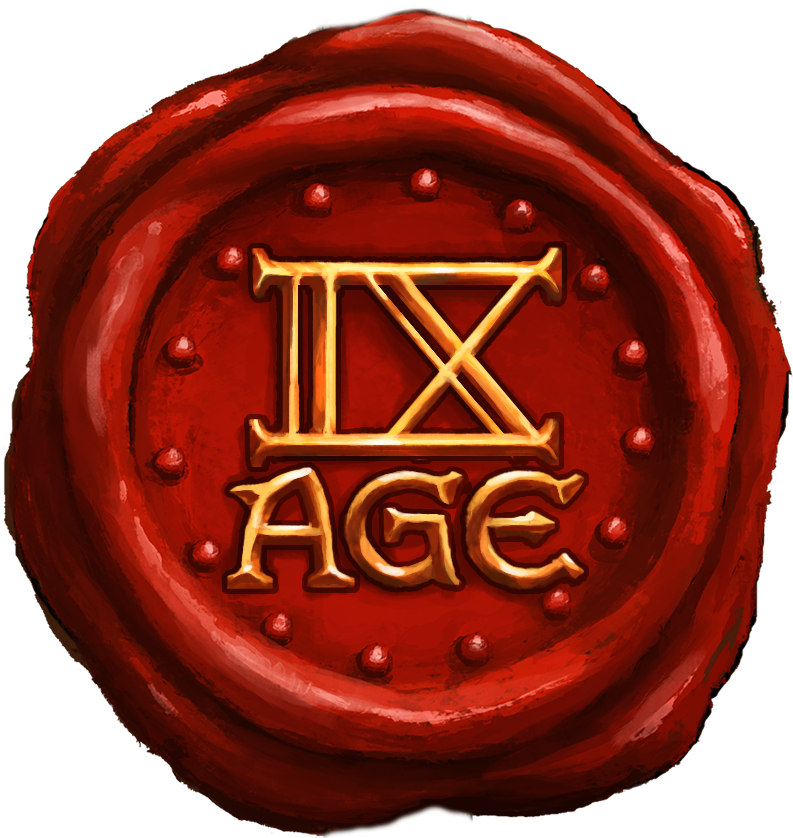
\includegraphics[width=2cm]{../Layout/pics/seal_9th.png} &
{\fontsize{10}{12}\selectfont \textcolor{black!50}{\noindent\labels@frontpagecredits}}

\ifdef{\frontpageaddstuff}{{\fontsize{10}{12}\selectfont \noindent\textcolor{black!50}{\frontpageaddstuff}}}{}

\vspace*{10pt}
\noindent{\fontsize{10}{12}\selectfont \textcolor{black!50}{\labels@license}}
\tabularnewline
\end{tabular}


\end{center}

\newpage

\thispagestyle{empty}

{\fontsize{10}{12}\selectfont

\begin{center}\hypertarget{tableofcontents}{\noindent{\Largerfontsize\textbf{\labels@tableofcontents}}}\end{center}

\vspace*{0.2cm}

\begin{center}
\noindent\hyperlink{howtousethisdoc}{\howtousethisdoc}
\end{center}

\begin{multicols}{2}

\tocentry{alchemy}{\alchemyTOC}

\tocentry{shamanism}{\shamanismTOC}

\tocentry{cosmology}{\cosmologyTOC}

\tocentry{divination}{\divinationTOC}

\tocentry{druidism}{\druidismTOC}

\tocentry{evocation}{\evocationTOC}

\tocentry{occultism}{\occultismTOC}

\tocentry{pyromancy}{\pyromancyTOC}

\tocentry{witchcraft}{\witchcraftTOC}

\tocentry{thaumaturgy}{\thaumaturgyTOC}

\end{multicols}

\begin{center}
\noindent\hyperlink{magicphasesummary}{\magicphasesummary}
\end{center}

\ifdef{\labels@introduction}{\vspace{0.7cm}\labels@introduction}{\vphantom{1pt}}
\vfill

\noindent\newrule{\labels@rulechanges}

\bigskip
\noindent \labels@latexcredit
}


\end{titlepage}

\restoregeometry

\basictitle{howtousethisdoc}{\howtousethisdoc}

Toutes les Voies de Magie sont présentées dans ce livre. Chaque Voie comprend un certain nombre de sorts. On tire en général au hasard au début de la partie les sorts que connaissent chaque \wizard{}, en utilisant les règles décrites dans le paragraphe \og Générer les Sorts \fg{} du Livre de Règles. Chaque \wizard{} doit choisir une Voie de Magie parmi celles auxquelles il a accès. Ce choix doit être indiqué dans la Liste d'Armée. Les sorts sont répartis en plusieurs catégories :

\vspace*{-10pt}
\begin{multicols}{2}

\basictitlenotoc{1-6}

\basicsubtitle{\learnedspells}

Ce sont les sorts numérotés entre 1 et 6. Ils n'ont pas d'effets particuliers en dehors de la façon dont ils sont générés (voir \og Générer les Sorts \fg{}).

\vspace*{-25pt}
\basictitlenotoc{\attributespellnumber}

\basicsubtitle{\attributespells}

Ce sont les sorts dont le label est un \og \attributespellnumber{} \fg{}. Tout \wizard{} qui génère au moins un Sort depuis une Voie connaît automatiquement l'\attributespell{}. Les \attributespells{} sont des sorts spéciaux qui ne peuvent pas être lancés indépendamment. Un lanceur peut s'il le souhaite lancer l'\attributespell{} à chaque fois qu'il lance avec succès un Sort non Attribut de la même Voie, après que l'effet du Sort a été résolu. Les Attributs ne peuvent pas être dissipés.

\columnbreak

\basictitlenotoc{0}

\basicsubtitle{\learnedspell{} 0}

Le \learnedspell{} numéroté 0 est un type spécial de \learnedspell{} qu'un \wizard{} peut obtenir en remplaçant un autre de ses \learnedspells{}.

\vspace*{-25pt}
\basictitlenotoc{\traitspellnumber}

\basicsubtitle{\traitspells}

Ce sont les sorts dont le label est un \og \traitspellnumber{} \fg{}. Ils n'ont pas d'effets particuliers en dehors de la façon dont ils sont générés : tout \wizard{} qui génère au moins un Sort d'une Voie connaît automatiquement le \traitspell{} de cette Voie.

\vspace*{\fill}
\end{multicols}

Les sorts sont définis par six propriétés :

\begin{multicols}{3}\raggedcolumns

\begin{center}
\basicsubtitle{Nom du Sort}

Utilisé pour nommer le sort que vous voulez lancer.

\basicsubtitle{\spellsEffect}

L'Effet détermine ce qui arrive à la cible quand le sort est lancé avec succès. Les Effets de sort ne sont jamais affectés par les règles spéciales, les Objets Magiques, les Effets d'autres sorts ou des capacités similaires qui donnent des bonus à la figurine qui lance le sort, à moins que le contraire ne soit précisé.
\end{center}

\vspace*{\fill}\columnbreak

\begin{center}
\basicsubtitle{\spellsType}

Le Type décrit les contraintes sur le choix des cibles du sort. Le Livre de Règles contient une description détaillée des Types de sort.

\basicsubtitle{\spellsDuration}

La Durée précise combien de temps sont appliqués les effets du sort. Le Livre de Règles contient une description détaillée des Durées de sort.
\end{center}
\vspace*{\fill}\columnbreak

\begin{center}
\basicsubtitle{Valeur de Lancement}

La Valeur de Lancement est la valeur minimale à atteindre pour réussir une tentative de lancement. Un sort peut posséder plusieurs Valeurs de Lancement (voir \og Sorts Améliorés \fg{}).

\basicsubtitle{\spellsRange}

La Portée donne la distance maximale entre le Lanceur du sort et sa cible.
\end{center}
\vspace*{\fill}
\end{multicols}

\vspace*{5pt}

\textbf{\Largerfontsize{}Sorts Améliorés}

\vspace*{5pt}

Certains sorts ont plusieurs Valeurs de Lancement, les Valeurs au-delà de la première étant appelées versions améliorées du sort. La Portée et les restrictions de cible des versions améliorées peuvent changer, voire les effets du sort : la Portée peut par exemple être augmentée. Déclarez si vous tentez de lancer une version améliorée, et laquelle, avant de lancer les dés. Si aucune déclaration n'est faite, on suppose qu'il s'agit de la version non améliorée du sort.

Les éléments du sort qui changent sur les versions améliorées et ceux qui restent identiques sont mis en valeur par un code couleur. Le \base{texte rouge} réfère à la version non améliorée du sort tandis que le \boosted{texte en bleu, gras et entre crochets} correspond à la version améliorée. Dans quelques rares cas, une seconde version améliorée ou une autre façon de lancer les sorts est disponible et est représentée en \secboosted{vert olive, gras et entre accolades}.



\newpathlogo{\alchemyicon}{alchemy}

\starttable{\colors@alchemy}{\alchemy}

\tablelabels

\spelllabelandtitle{\attributespellnumber}{\alchemyattribute}

\tablespellcastingvalue{}
\tablespellrange{\distance{18}}
\tablespelltype{\hex}
\tablespellduration{\lastsoneturn}
\tablespelleffect{%
La cible gagne la règle \flammable{} contre les Attaques de Corps à Corps et les Sorts.
}
\hline
\spelllabelandtitle{0}{\alchemyspellzero}

\tablespellcastingvalue{8+}
\tablespellrange{\distance{24}}
\tablespelltype{\hex\newline\missile\newline\damage}
\tablespellduration{\instant}
\tablespelleffect{%
La cible subit 1D3+1 touches avec la règle \metalshifting{}.
}
\hline
\spelllabelandtitle{1}{\alchemyspellone}

\tablespellcastingvalue{\base{6+}\newline\boosted{9+}}
\tablespellrange{\base{\distance{24}}\newline\boosted{\distance{48}}}
\tablespelltype{\augment}
\tablespellduration{\lastsoneturn}
\tablespelleffect{%
La cible gagne +1 à sa Sauvegarde d'Armure.
}
\hline
\spelllabelandtitle{2}{\alchemyspelltwo}

\tablespellcastingvalue{\base{7+}\newline\boosted{10+}}
\tablespellrange{\distance{24}}
\tablespelltype{\hex\newline\missile\newline\damage}
\tablespellduration{\instant}
\tablespelleffect{%
La cible subit \base{2D6} \boosted{3D6} touches de Force 2 avec les règles \flamingattacks{} et \armourpiercing{3}.
}
\hline
\spelllabelandtitle{3}{\alchemyspellthree}

\tablespellcastingvalue{\base{8+}\newline\boosted{11+}}
\tablespellrange{\base{\distance{24}}\newline\boosted{\distance{48}}}
\tablespelltype{\hex}
\tablespellduration{\permanent}
\tablespelleffect{%
La cible subit un malus de -1 à sa Sauvegarde d'Armure.
}
\hline
\spelllabelandtitle{4}{\alchemyspellfour}

\tablespellcastingvalue{\base{8+}\newline\boosted{11+}}
\tablespellrange{\base{\distance{18}}\newline\boosted{\distance{36}}}
\tablespelltype{\hex\newline\missile\newline\damage}
\tablespellduration{\instant}
\tablespelleffect{%
La cible subit une touche de Force 6 avec les règles \penetrating{}, \multiplewounds{1D3}{} et \armourpiercing{6}.
}
\hline
\spelllabelandtitle{5}{\alchemyspellfive}

\tablespellcastingvalue{\base{9+}\newline\boosted{12+}}
\tablespellrange{\base{\distance{24}}\newline\boosted{\distance{48}}}
\tablespelltype{\hex}
\tablespellduration{\lastsoneturn}
\tablespelleffect{%
Les attaques de la cible ne peuvent pas bénéficier de bonus de Force de ses Armes de Corps à Corps. Les Armes de Tir standard maniées par la cible subissent un malus de -1 en Force. Ce sort n'affecte que la Force et l'équipement des figurines, pas leurs règles spéciales.
}
\hline
\spelllabelandtitle{6}{\alchemyspellsix}

\tablespellcastingvalue{10+}
\tablespellrange{\distance{18}}
\tablespelltype{\augment}
\tablespellduration{\lastsoneturn}
\tablespelleffect{%
La cible gagne les règles \flamingattacks{}, \magicalattacks{} et \armourpiercing{+1}.
}

\closetable{}



\newpathlogo{\shamanismicon}{shamanism}

\starttable{\colors@shamanism}{\textcolor{white}{\shamanism}}

\tablelabels

\spelllabelandtitle{\attributespellnumber}{\shamanismattribute}

\tablespellcastingvalue{}
\tablespellrange{\caster}
\tablespelltype{}
\tablespellduration{\lastsoneturn}
\tablespelleffect{%
Les Attaques de Corps à Corps dirigées contre la cible ne peuvent pas blesser sur mieux que 5+.
}
\hline
\spelllabelandtitle{0}{\shamanismspellzero}

\tablespellcastingvalue{\base{6+}\newline\boosted{8+}}
\tablespellrange{\distance{18}}
\tablespelltype{\augment}
\tablespellduration{\lastsoneturn}
\tablespelleffect{%
La cible gagne +1 en \base{Force} \boosted{Endurance}.
}
\hline
\spelllabelandtitle{1}{\shamanismspellone}

\tablespellcastingvalue{\base{5+}\newline\boosted{8+}}
\tablespellrange{\base{\distance{24}}\newline\boosted{\distance{48}}}
\tablespelltype{\hex\newline\missile\newline\damage}
\tablespellduration{\instant}
\tablespelleffect{%
La cible subit 5D6 touches de Force 1.
}
\hline
\spelllabelandtitle{2}{\shamanismspelltwo}

\tablespellcastingvalue{\base{5+}\newline\boosted{9+}}
\tablespellrange{\base{\distance{6}}\newline\boosted{\distance{18}}}
\tablespelltype{\universal}
\tablespellduration{\lastsoneturn}
\tablespelleffect{%
La cible gagne la règle \frenzy{}.
}
\hline
\spelllabelandtitle{3}{\shamanismspellthree}

\tablespellcastingvalue{\base{5+}\newline\boosted{9+}}
\tablespellrange{\base{\distance{18}}\newline\boosted{\aura{} \distance{12}}}
\tablespelltype{\augment}
\tablespellduration{\instant}
\tablespelleffect{%
La cible effectue un Mouvement Magique de \distance{2D6} droit devant. Elle ne peut pas se déplacer en arrière, sur le côté, se reformer, faire un Pivot ou une Roue pendant ce mouvement. Elle peut cependant choisir de ne pas se déplacer, ou de ne parcourir qu'une partie de la distance.\newline
\boosted{Si plusieurs unités sont affectées, faites le jet de distance et déplacez une unité avant de vous préoccuper de la suivante.}
}
\hline
\spelllabelandtitle{4}{\shamanismspellfour}

\tablespellcastingvalue{\base{7+}\newline\boosted{10+}}
\tablespellrange{\base{\distance{18}}\newline\boosted{\aura{} \distance{12}}}
\tablespelltype{\augment}
\tablespellduration{\lastsoneturn}
\tablespelleffect{%
Les jets pour blesser des Attaques de Tir dirigées contre la cible subissent un malus de -1.
}
\hline
\spelllabelandtitle{5}{\shamanismspellfive}

\tablespellcastingvalue{\base{9+}\newline\boosted{12+}}
\tablespellrange{\base{\distance{36}}\newline\boosted{\distance{72}}}
\tablespelltype{\hex}
\tablespellduration{\lastsoneturn}
\tablespelleffect{%
La cible subit un malus de -1 pour toucher et traite tous les terrains, y-compris les Terrains Découverts, comme des Terrains Dangereux (2).
}
\hline
\spelllabelandtitle{6}{\shamanismspellsix}

\tablespellcastingvalue{\base{10+}\newline\boosted{13+}}
\tablespellrange{\distance{96}}
\tablespelltype{\ground}
\tablespellduration{\instant}
\tablespelleffect{%
Invoque une \totemicbeast{} (caractéristiques ci-dessous). Elle doit être placée à \base{\distance{1}} \boosted{\distance{10}} d'un bord de table.
}

\closetable{}

\vspace*{10pt}
{\largerfontsize{\textbf{\totemicbeast}}} \textbf{(pour l'\shamanismspellsix{})}

{
\setlength{\tabcolsep}{6pt}
\renewcommand{\arraystretch}{1.5}
\begin{tabular}{p{1.5cm}ccccccccc>{\raggedleft}p{4cm}}
\hline
\normalfontsize & \normalfontsize\labels@M{} & \normalfontsize\labels@WS{} & \normalfontsize\labels@BS{} & \normalfontsize\labels@S{} & \normalfontsize\labels@T{} & \normalfontsize\labels@W{} & \normalfontsize\labels@I{} & \normalfontsize\labels@A{} & \normalfontsize\labels@Ld{} & \largefontsize\monstrousbeast{} \tabularnewline
\largefontsize & 3D6 & 3 & - & 5 & 5 & 3 & 3 & 4 & 7 & \labels@basesize{} \unit{40x40}{\milli\meter} \tabularnewline
\end{tabular}
}

\textit{\normalfontsize\labels@specialrules}\spacebeforecolon{}: \breathweapon{\Strength{} 3}, \immunetopsychology{}, \randommovement{3D6}


\newcosmologylogo

{
\renewcommand{\arraystretch}{1.65}
\starttablecosmology

\tablepassivecosmology{\cosmologypassive}{Les sorts de la \cosmology{} sont divisés en deux versions : \textbf{\cosmos} et \textbf{\chaos}. Déclarez quelle version du sort vous utilisez au lancement.\newline
Quand un sort de la \cosmology{} est lancé avec succès et que le lanceur ne dispose pas de compteur \cosmology{}, il gagne un compteur correspondant à la version du sort choisie : \textbf{\cosmos} ou \textbf{\chaos}.\newline
La valeur de lancement des sorts non liés à des \boundspells{} de la \cosmology{} est \secboosted{réduite de 2} quand ils sont lancés par un \wizard{} qui possède un compteur \cosmology{} correspondant à la version du sort qui est lancée. Par exemple la version \textbf{\cosmos} d'un sort a une valeur de lancement réduite si le Lanceur possède un compteur \textbf{\cosmos}. Un \wizard{} qui tente de lancer un sort de la \cosmology{} dont la version ne correspond pas à celle de son compteur perd immédiatement ce compteur.\newline
À la fin de chacune de vos Phases de Magie, remplacez tous vos compteurs \textbf{\cosmos} par des compteurs \textbf{\chaos}, et tous les compteurs \textbf{\chaos} par des \textbf{\cosmos}.}

\tablelabelscosmology

\spelllabelandtitlecosmology{0}{\cosmologyspellzero}
\tablespellcastingvaluecosmology{8+}{6+}
\tablespellrangecosmology{\distance{24}}
\tablecosmosicon{}
\textbf{\augment}&
\multirow{2}{*}{\lastsoneturn}&
\tablespelltextcosmology{La cible gagne \textbf{+1} en Capacité de Combat et \textbf{+1} en Capacité de Tir.}
\tablechaosicon{}
\textbf{\hex}&
&
\tablespelltextcosmology{La cible subit un malus de \textbf{-1} en CC, jusqu'à un minimum de 1, et de \textbf{-1} en CT.}
\hline

\spelllabelandtitlecosmology{1}{\cosmologyspellone}
\tablespellcastingvaluecosmology{7+}{5+}
\tablespellrangecosmology{\distance{18}}
\tablecosmosicon{}
\focused{},\newline\textbf{\augment}&
\multirow{2}{*}{\vspace*{-0.6cm}\instant}&
\tablespelltextcosmology{La cible \textbf{Récupère} 1 Point de Vie.}
\tablechaosicon{}
\focused{},\newline\textbf{\hex},\newline\textbf{\direct}, \textbf{\damage}&
&
\tablespelltextcosmology{La cible subit une touche qui blesse automatiquement avec la règle \armourpiercing{6}.}
\hline

\spelllabelandtitlecosmology{2}{\cosmologyspelltwo}
\tablespellcastingvaluecosmology{7+}{5+}
\tablespellrangecosmology{\distance{18}}
\tablecosmosicon{}
\textbf{\augment}&
\multirow{2}{*}{\vspace*{-0.2cm}\remainsinplay}&
\tablespelltextcosmology{La cible gagne \textbf{+1} en Commandement.}
\tablechaosicon{}
\textbf{\hex}&
&
\tablespelltextcosmology{La cible subit un malus de \textbf{-1} en Commandement.}
\hline

\spelllabelandtitlecosmology{3}{\cosmologyspellthree}
\tablespellcastingvaluecosmology{9+}{7+}
\tablespellrangecosmology{\distance{18}}
\tablecosmosicon{}
\textbf{\augment}&
\multirow{2}{*}{\vspace*{-0.5cm}\lastsoneturn}&
\tablespelltextcosmology{La cible jette un dé additionnel et ignore celui ayant donné le résultat le plus \textbf{petit} pour la Charge, Charge Irrésistible, Fuite et Poursuite.}
\tablechaosicon{}
\textbf{\hex}&
&
\tablespelltextcosmology{La cible jette un dé additionnel et ignore celui ayant donné le résultat le plus \textbf{grand} pour la Charge, Charge Irrésistible, Fuite et Poursuite.}
\hline

\spelllabelandtitlecosmology{4}{\cosmologyspellfour}
\tablespellcastingvaluecosmology{9+}{7+}
\tablespellrangecosmology{\distance{18}}
\tablecosmosicon{}
\multirow{2}{2.5cm}{\vspace*{-0.22cm}\newline\hex{},\newline\missile{},\newline\damage}&
\multirow{2}{*}{\vspace*{-0.3cm}\instant}&
\tablespelltextcosmology{La cible subit 2D6 touches de Force 3 avec les règles \textbf{\divineattacks{} et \flamingattacks{}}.}
\tablechaosicon{}
&
&
\tablespelltextcosmology{La cible subit 2D6 touches de Force 3 avec la règle \textbf{\armourpiercing{3}}.}
\hline

\spelllabelandtitlecosmology{5}{\cosmologyspellfive}
\tablespellcastingvaluecosmology{10+}{8+}
\tablespellrangecosmology{\distance{18}}
\tablecosmosicon{}
\textbf{\augment}&
\multirow{2}{*}{\vspace*{-0.2cm}\lastsoneturn}&
\tablespelltextcosmology{La cible gagne \textbf{+1} en Force.}
\tablechaosicon{}
\textbf{\hex}&
&
\tablespelltextcosmology{La cible subit un malus de \textbf{-1} en Force.}
\hline

\spelllabelandtitlecosmology{6}{\cosmologyspellsix}
\tablespellcastingvaluecosmology{11+}{9+}
\tablespellrangecosmology{\distance{18}}
\tablecosmosicon{}
\textbf{\augment}&
\textbf{\lastsoneturn}&
\tablespelltextcosmology{Toutes les figurines de l'unité ciblée \textbf{gagnent une \wardsave{5}}.}
\tablechaosicon{}
\textbf{\hex},\newline\textbf{\direct}, \textbf{\damage}&
\textbf{\instant}&
\tablespelltextcosmology{Toutes les figurines de l'unité ciblée \textbf{subissent une touche de Force 3}.}

\closetable{}
}








\newpathlogo{\divinationicon}{divination}

\starttable{\colors@divination}{\divination}

\tablepassive{\divinationpassive}{Les Sorts de la \divination{} gagnent un bonus de \distance{+3} en Portée pour chaque autre \wizard{} à moins de \distance{12} du Lanceur avec des Sorts de la \divination{} ne provenant pas d'\boundspells{}. Quand un \wizard{} qui tente de lancer un sort de la \divination{} subit une \lostfocus{}, tous les autres \wizards{} alliés à moins de \distance{12} du Lanceur avec des Sorts de la \divination{} ne provenant pas d'\boundspells{} subissent aussi une \lostfocus{}, jusqu'à la fin de la Phase de Magie.}

\hline
\tablelabels

\spelllabelandtitle{\attributespellnumber}{\divinationattribute}

\tablespellcastingvalue{}
\tablespellrange{\distance{18}}
\tablespelltype{\augment}
\tablespellduration{\lastsoneturn}
\tablespelleffect{%
Jetez un dé supplémentaire et ignorez le dé avec le plus grand résultat quand la cible passe un Test de Commandement.\newline
Une unité ne peut être affectée par ce sort qu'une seule fois par Phase de Magie.
}
\hline
\spelllabelandtitle{0}{\divinationspellzero}

\tablespellcastingvalue{\base{7+}\newline\boosted{10+}}
\tablespellrange{\base{\distance{18}}\newline\boosted{\aura{} \distance{6}}}
\tablespelltype{\augment}
\tablespellduration{\lastsoneturn}
\tablespelleffect{%
La cible gagne les règles \hardtarget{} et \distracting{}.
}
\hline
\spelllabelandtitle{1}{\divinationspellone}

\tablespellcastingvalue{\base{7+}\newline\boosted{10+}}
\tablespellrange{\distance{18}}
\tablespelltype{\hex\newline\missile\newline\damage}
\tablespellduration{\instant}
\tablespelleffect{%
La cible subit \base{1D3} \boosted{1D6} touches qui blessent automatiquement et contre lesquelles aucune \wardsave{} ou de \regeneration{} n'est permise.
}
\hline
\spelllabelandtitle{2}{\divinationspelltwo}

\tablespellcastingvalue{\base{8+}\newline\boosted{12+}}
\tablespellrange{\base{\distance{18}}\newline\boosted{\aura{} \distance{6}}}
\tablespelltype{\augment}
\tablespellduration{\lastsoneturn}
\tablespelleffect{%
La cible gagne +2 en Capacité de Combat et en Initiative.
}
\hline
\spelllabelandtitle{3}{\divinationspellthree}

\tablespellcastingvalue{\base{9+}\newline\boosted{12+}}
\tablespellrange{\base{\distance{18}}\newline\boosted{\aura{} \distance{6}}}
\tablespelltype{\augment}
\tablespellduration{\lastsoneturn}
\tablespelleffect{%
La cible gagne la règle \divineattacks{} et doit relancer les jets pour toucher ratés de ses Attaques de Corps à Corps \base{et de Tir}.
}
\hline
\spelllabelandtitle{4}{\divinationspellfour}

\tablespellcastingvalue{9+}
\tablespellrange{\distance{18}}
\tablespelltype{\augment}
\tablespellduration{\lastsoneturn}
\tablespelleffect{%
La cible gagne les règles \immunetopsychology{} et \stubborn{}.
}
\hline
\spelllabelandtitle{5}{\divinationspellfive}

\tablespellcastingvalue{\base{9+}\newline\boosted{13+}}
\tablespellrange{\distance{18}}
\tablespelltype{\hex\newline\missile\newline\damage}
\tablespellduration{\instant}
\tablespelleffect{%
La cible subit \base{2D6} \boosted{3D6} touches qui blessent sur 4+ avec les règles \divineattacks{} et \armourpiercing{2}.
}
\hline
\spelllabelandtitle{6}{\divinationspellsix}

\tablespellcastingvalue{10+}
\tablespellrange{\distance{18}}
\tablespelltype{\hex}
\tablespellduration{\lastsoneturn}
\tablespelleffect{%
Au début de chacune des phases suivantes, lancez 1D6 plus 1D6 par Personnage dans l'unité ciblée. Si au moins l'un des dés donne un \result{6}, la cible ne peut effectuer l'action correspondante pendant cette phase.

\vspace*{10pt}
\textbf{Étape de Déclaration des Charges} : Déclarer des Charges.\newline
\textbf{Étape des Autres Mouvements} : Faire une Marche Forcée.\newline
\textbf{Phase de Magie} : Lancer des Sorts.\newline
\textbf{Phase de Tir} : Tirer.
}

\closetable{}


\newpathlogo{\druidismicon}{druidism}

\starttable{\colors@druidism}{\druidism}

\tablelabels

\spelllabelandtitle{\attributespellnumber}{\druidismattribute}

\tablespellcastingvalue{}
\tablespellrange{\distance{12}}
\tablespelltype{\focused\newline\augment}
\tablespellduration{\instant}
\tablespelleffect{%
La cible ou son unité Récupère \secboosted{Ressuscite} 1 Point de Vie. Aucune figurine ne peut Récupérer (ou Ressusciter) plus d'un Point de Vie par phase grâce à ce sort.
}
\hline
\spelllabelandtitle{\traitspellnumber}{\druidismtraitspell}

\tablespellcastingvalue{4+}
\tablespellrange{\caster}
\tablespelltype{}
\tablespellduration{\remainsinplay}
\tablespelleffect{%
Si le Lanceur a ce sort en jeu quand il lance d'autres sorts de cette Voie, la version améliorée des sorts, marquée par \secboosted{ }, est utilisée. Pour l'Attribut de la Voie, \druidismtraitspell{} doit être en jeu quand le sort déclenchant l'Attribut est lancé.
}
\hline
\spelllabelandtitle{1}{\druidismspellone}

\tablespellcastingvalue{6+}
\tablespellrange{\distance{18}}
\tablespelltype{\hex\newline\direct\newline\damage}
\tablespellduration{\instant}
\tablespelleffect{%
La Portée de ce sort peut être mesurée depuis le lanceur ou depuis n'importe quel décor de \textbf{\impassableterrain} de la table.\newline
La cible subit 1D6 touches de Force 4 \secboosted{5}.
}
\hline
\spelllabelandtitle{2}{\druidismspelltwo}

\tablespellcastingvalue{8+}
\tablespellrange{\distance{12}}
\tablespelltype{\augment}
\tablespellduration{\lastsoneturn}
\tablespelleffect{%
La Portée de ce sort peut être mesurée depuis le lanceur ou depuis n'importe quel décor d'\textbf{\water} de la table.\newline
La cible gagne la règle \regeneration{5} \secboosted{(4+)}.
}
\hline
\spelllabelandtitle{3}{\druidismspellthree}

\tablespellcastingvalue{8+}
\tablespellrange{\distance{12}}
\tablespelltype{\hex}
\tablespellduration{\lastsoneturn}
\tablespelleffect{%
La Portée de ce sort peut être mesurée depuis le lanceur ou depuis n'importe quel décor de \textbf{\forest} de la table.\newline
La cible subit un malus de -1 \secboosted{-1D3} en Capacité de Combat et en Capacité de Tir, jusqu'à un minimum de 1.
}
\hline
\spelllabelandtitle{4}{\druidismspellfour}

\tablespellcastingvalue{9+}
\tablespellrange{\distance{12}}
\tablespelltype{\augment\newline\secboosted{\universal}}
\tablespellduration{\lastsoneturn}
\tablespelleffect{%
Toutes les figurines de l'unité ciblée sont considérées comment se trouvant dans une \forest{}.\newline
\secboosted{Si la cible est une unité alliée, elle gagne la règle \strider{\forest}.}
}
\hline
\spelllabelandtitle{5}{\druidismspellfive}

\tablespellcastingvalue{11+}
\tablespellrange{\distance{12}}
\tablespelltype{\augment}
\tablespellduration{\lastsoneturn}
\tablespelleffect{%
La Portée de ce sort peut être mesurée depuis le lanceur ou depuis n'importe quel décor de \textbf{Colline} de la table.\newline
La cible gagne +2 \secboosted{+3} Endurance.
}
\hline
\spelllabelandtitle{6}{\druidismspellsix}

\tablespellcastingvalue{11+}
\tablespellrange{\distance{24}}
\tablespelltype{\augment}
\tablespellduration{\instant}
\tablespelleffect{%
Ce sort a un effet différent selon la Taille de la plus grande fraction des figurines de l'unité ciblée. Utilisez l'effet de la plus grande Taille en cas d'égalité.\newline
\textbf{Standard} : Ressuscite 1D3+3 \secboosted{1D3+5} Points de Vie.\newline
\textbf{Grande} : Ressuscite 1D3 \secboosted{1D3+1} Points de Vie.\newline
\textbf{Gigantesque} : Ressuscite 1 \secboosted{1} Point de Vie.
}

\closetable{}


\newpathlogo{\evocationicon}{evocation}

\starttable{\colors@evocation}{\textcolor{white}{\evocation}}

\tablelabels

\spelllabelandtitle{\traitspellnumber}{\evocationtraitspell}

\tablespellcastingvalue{\base{5+}\newline\boosted{8+}}
\tablespellrange{\base{\distance{18}}\newline\boosted{\aura{} \distance{6}}}
\tablespelltype{\augment}
\tablespellduration{\instant\vspace*{25pt}\newline\lastsoneturn}
\tablespelleffect{%
\textbf{Si la cible possède au moins une figurine avec une valeur \evoked{} :}\newline
L'unité ciblée ou un unique Personnage dans l'unité ciblée Ressuscite un nombre de Points de Vie correspondant à la valeur d'\evoked{} précisée dans son profil.\vspace*{5pt}\newline
\textbf{Si la cible ne possède pas de figurine avec une valeur \evoked{} :}\newline
L'unité ciblée gagne les règles \immunetopsychology{} et \fear{}.
}
\hline
\spelllabelandtitle{1}{\evocationspellone}

\tablespellcastingvalue{\base{5+}\newline\boosted{10+}}
\tablespellrange{\base{\distance{18}}\newline\boosted{\aura{} \distance{12}}}
\tablespelltype{\augment}
\tablespellduration{\lastsoneturn}
\tablespelleffect{%
La cible gagne la règle \lethalstrike{}. Les Attaques qui bénéficiaient déjà de cette règle peuvent relancer leurs jets pour blesser ratés au Corps à Corps.
}
\hline
\spelllabelandtitle{2}{\evocationspelltwo}

\tablespellcastingvalue{\base{7+}\newline\boosted{9+}}
\tablespellrange{\distance{12}}
\tablespelltype{\augment}
\tablespellduration{\lastsoneturn}
\tablespelleffect{%
La cible doit relancer ses jets pour toucher des Attaques de Corps à Corps \boosted{et de Tir}.
}
\hline
\spelllabelandtitle{3}{\evocationspellthree}

\tablespellcastingvalue{\base{7+}\newline\boosted{10+}}
\tablespellrange{\base{\distance{12}}\newline\boosted{\distance{24}}}
\tablespelltype{\focused\newline\hex\newline\direct\newline\damage}
\tablespellduration{\instant}
\tablespelleffect{%
La cible subit 1D3 touches de Force 10 avec la règle \armourpiercing{6}. Utilisez le Commandement de la cible à la place de son Endurance pour les jets pour blesser.
}
\hline
\spelllabelandtitle{4}{\evocationspellfour}

\tablespellcastingvalue{\base{7+}\newline\boosted{12+}}
\tablespellrange{\base{\distance{12}}\newline\boosted{\aura{} \distance{12}}}
\tablespelltype{\augment}
\tablespellduration{\instant}
\tablespelleffect{%
La cible peut effectuer un Mouvement Magique de \distance{8}. Elle compte comme ayant la règle \ethereal{} pendant ce déplacement.
}
\hline
\spelllabelandtitle{5}{\evocationspellfive}

\tablespellcastingvalue{9+}
\tablespellrange{\distance{24}}
\tablespelltype{\hex}
\tablespellduration{\remainsinplay}
\tablespelleffect{%
La cible subit un malus de -1 en Commandement et de -2 en Capacité de Combat, jusqu'à un minimum de 1.
}
\hline
\spelllabelandtitle{6}{\evocationspellsix}

\tablespellcastingvalue{14+}
\tablespellrange{\distance{18}}
\tablespelltype{\hex\newline\direct\newline\damage}
\tablespellduration{\instant}
\tablespelleffect{%
Chaque Personnage et Champion de l'unité ciblée subit une touche qui blesse automatiquement sans sauvegarde d'aucune sorte possible.
}

\closetable{}


\newpathlogo{\occultismicon}{occultism}

\starttable{\colors@occultism}{\textcolor{white}{\occultism}}

\tablepassive{\occultismpassive}{Quand un Sort de cette Voie non lié à un \boundspell{} est lancé, après avoir jeté les Dés de Magie mais avant que l'adversaire n'effectue une tentative de dissipation, le Joueur Actif peut choisir d'infliger X touches à l'unité du Lanceur ou à une autre unité alliée non engagée au Corps à Corps à moins de \distance{24}. Une unité ne peut être ciblée qu'une seule fois par cette capacité lors d'une Phase de Magie.\newline
X est égal au nombre de rangs de l'unité ciblée avec un minimum de 2 et un maximum de 5. Ces touches blessent automatiquement sans sauvegarde d'aucune sorte possible. La dernière figurine d'une unité ne peut jamais être retirée comme perte à cause de cette capacité : toute blessure qui réduirait sa Réserve de Points de Vie à 0 est ignorée.\newline
Si au moins une blessure est infligée, le sort est lancé avec la version améliorée marquée avec \secboosted{ }.}

\hline
\tablelabels

\spelllabelandtitle{0}{\occultismspellzero}

\tablespellcastingvalue{8+}
\tablespellrange{\aura{} \distance{12}}
\tablespelltype{\universal}
\tablespellduration{\instant}
\tablespelleffect{%
La cible subit 1D6 touches de Force 4. L'unité du Lanceur n'est pas affectée.\newline
\secboosted{Le Lanceur Récupère un PV si au moins une blessure non sauvegardée est infligée par ce sort.}
}
\hline
\spelllabelandtitle{1}{\occultismspellone}

\tablespellcastingvalue{6+}
\tablespellrange{\caster}
\tablespelltype{}
\tablespellduration{\lastsoneturn}
\tablespelleffect{%
La cible gagne une \wardsave{5}. La \wardsave{} des figurines affectées qui en possédaient déjà une est améliorée d'un point jusqu'à obtenir 3+ au mieux.
}
\hline
\spelllabelandtitle{2}{\occultismspelltwo}

\tablespellcastingvalue{6+}
\tablespellrange{\caster}
\tablespelltype{\focused}
\tablespellduration{\lastsoneturn}
\tablespelleffect{%
La cible gagne une \breathweapon{\toxicattacks}.
}
\hline
\spelllabelandtitle{3}{\occultismspellthree}

\tablespellcastingvalue{7+}
\tablespellrange{\caster}
\tablespelltype{}
\tablespellduration{\remainsinplay}
\tablespelleffect{%
La cible peut relancer ses jets de lancement de sort quand elle lance des sorts non liés à des \boundspells{} de cette Voie.
}
\hline
\spelllabelandtitle{4}{\occultismspellfour}

\tablespellcastingvalue{9+}
\tablespellrange{\distance{24}}
\tablespelltype{\hex}
\tablespellduration{\permanent}
\tablespelleffect{%
La cible subit un malus de -1 en Capacité de Combat, jusqu'à un minimum de 1.\newline
\secboosted{Le Lanceur gagne +1 en Capacité de Combat.}
}
\hline
\spelllabelandtitle{5}{\occultismspellfive}

\tablespellcastingvalue{10+}
\tablespellrange{\distance{18}}
\tablespelltype{\hex\newline\direct\newline\damage}
\tablespellduration{\instant}
\tablespelleffect{%
La cible subit une touche de Force 10 avec la règle \multiplewounds{1D3}{}.\newline
\secboosted{Le Lanceur peut choisir de cibler un unique Personnage de l'unité ciblée.}
}
\hline
\spelllabelandtitle{6}{\occultismspellsix}

\tablespellcastingvalue{12+}
\tablespellrange{\distance{12}}
\tablespelltype{\hex\newline\direct\newline\damage}
\tablespellduration{\instant}
\tablespelleffect{%
La cible subit 2D6 touches de Force 5.\newline
\secboosted{La Force des touches passe à 6.}
}

\closetable{}


\newpathlogo{\pyromancyicon}{pyromancy}

\starttable{\colors@pyromancy}{\textcolor{white}{\pyromancy}}

\tablelabels

\spelllabelandtitle{\traitspellnumber}{\pyromancytraitspell}

\tablespellcastingvalue{4+}
\tablespellrange{\distance{24}}
\tablespelltype{\hex\newline\missile\newline\damage}
\tablespellduration{\instant}
\tablespelleffect{%
La cible subit 1D3+1 touches de Force 4 avec la règle \flamingattacks{}.
}
\hline
\spelllabelandtitle{1}{\pyromancyspellone}

\tablespellcastingvalue{\base{5+}\newline\boosted{9+}\newline\secboosted{12+}}
\tablespellrange{\base{\distance{36}}\newline\boosted{\distance{24}}\newline\secboosted{\distance{12}}}
\tablespelltype{\hex\newline\missile\newline\damage}
\tablespellduration{\instant}
\tablespelleffect{%
La cible subit \base{1D6} \boosted{2D6} \secboosted{3D6} touches de Force 4 avec la règle \flamingattacks{}.
}
\hline
\spelllabelandtitle{2}{\pyromancyspelltwo}

\tablespellcastingvalue{\base{6+}\newline\boosted{10+}}
\tablespellrange{\base{\distance{24}}\newline\boosted{\aura{} \distance{6}}}
\tablespelltype{\augment}
\tablespellduration{\remainsinplay}
\tablespelleffect{%
Toutes les figurines ennemies en contact socle à socle avec l'unité ciblée subissent une touche de Force 4 avec la règle \flamingattacks{} au palier d'Initiative 0 de chaque Manche de Corps à Corps impliquant la cible. Cela compte comme une Attaque Spéciale de Corps à Corps.
}
\hline
\spelllabelandtitle{3}{\pyromancyspellthree}

\tablespellcastingvalue{\base{7+}\newline\boosted{10+}}
\tablespellrange{\aura{} \distance{18}}
\tablespelltype{\hex\newline\damage}
\tablespellduration{\instant}
\tablespelleffect{%
La cible subit \base{1D3} \boosted{1D6} touches de Force 4 avec la règle \flamingattacks{}.
}
\hline
\spelllabelandtitle{4}{\pyromancyspellfour}

\tablespellcastingvalue{8+}
\tablespellrange{\distance{18}}
\tablespelltype{\ground}
\tablespellduration{\remainsinplay}
\tablespelleffect{%
Placez le centre d'un gabarit rond de \distance{3} de diamètre sur le point ciblé. Le gabarit doit se trouver à plus de \distance{1} de toute unité.\newline
À la fin de chaque Phase, toute unité qui a été en contact avec le gabarit pendant la phase subit une \areaattack{4} de Force 4 avec la règle \flamingattacks{}. Une unité ne peut être affectée par ce sort qu'une seule fois par Tour de Joueur.
}
\hline
\spelllabelandtitle{5}{\pyromancyspellfive}

\tablespellcastingvalue{\base{10+}\newline\boosted{13+}}
\tablespellrange{\base{\distance{18}}\newline\boosted{\aura{} \distance{6}}}
\tablespelltype{\augment}
\tablespellduration{\lastsoneturn}
\tablespelleffect{%
Les Attaques de Corps à Corps et de Tir de la cible gagnent un bonus de +1 pour blesser et les règles \flamingattacks{} et \magicalattacks{}.
}
\hline
\spelllabelandtitle{6}{\pyromancyspellsix}

\tablespellcastingvalue{12+}
\tablespellrange{\distance{24}}
\tablespelltype{\hex\newline\direct\newline\damage}
\tablespellduration{\instant}
\tablespelleffect{%
Chaque figurine de l'unité ciblée subit une touche de Force 3 avec la règle \flamingattacks{}.
}

\closetable{}


\newpathlogo{\witchcrafticon}{witchcraft}

\starttable{\colors@witchcraft}{\textcolor{white}{\witchcraft}}

\tablelabels

\spelllabelandtitle{0}{\witchcraftspellzero}

\tablespellcastingvalue{6+}
\tablespellrange{\distance{36}}
\tablespelltype{\hex}
\tablespellduration{\lastsoneturn}
\tablespelleffect{%
La cible subit un malus de -1D3 en Mouvement, jusqu'à un minimum de 3, et un malus de -1 en Initiative jusqu'à un minimum de 1.
}
\hline
\spelllabelandtitle{1}{\witchcraftspellone}

\tablespellcastingvalue{\base{5+}\newline\boosted{8+}}
\tablespellrange{\base{\distance{18}}\newline\boosted{\aura{} \distance{6}}}
\tablespelltype{\augment}
\tablespellduration{\lastsoneturn}
\tablespelleffect{%
La cible gagne les règles \hardtarget{} et \distracting{}.
}
\hline
\spelllabelandtitle{2}{\witchcraftspelltwo}

\tablespellcastingvalue{\base{6+}\newline\boosted{9+}}
\tablespellrange{\distance{18}}
\tablespelltype{\augment}
\tablespellduration{\instant}
\tablespelleffect{%
La cible peut effectuer un Mouvement Magique de \base{\distance{6}} \boosted{\distance{10}} avec la règle \fly{}. Elle peut se reformer avant et après le mouvement. Cela ne l'empêche pas de tirer par la suite.
}
\hline
\spelllabelandtitle{3}{\witchcraftspellthree}

\tablespellcastingvalue{\base{7+}\newline\boosted{10+}}
\tablespellrange{\base{\distance{36}}\newline\boosted{\distance{24}}}
\tablespelltype{\hex}
\tablespellduration{\lastsoneturn}
\tablespelleffect{%
La portée des Attaques de Tir effectuées par la cible \boosted{et des sorts lancés par la cible} est divisée par deux.
}
\hline
\spelllabelandtitle{4}{\witchcraftspellfour}

\tablespellcastingvalue{8+}
\tablespellrange{\distance{18}}
\tablespelltype{\universal}
\tablespellduration{\lastsoneturn}
\tablespelleffect{%
La cible gagne la règle \randommovement{2D6}.
}
\hline
\spelllabelandtitle{5}{\witchcraftspellfive}

\tablespellcastingvalue{8+}
\tablespellrange{\distance{24}}
\tablespelltype{\hex}
\tablespellduration{\remainsinplay}
\tablespelleffect{%
La cible gagne la règle \stupidity{}. Elle subit un malus de -1 en Commandement pour ses Tests de \stupidity{} pour chaque Personnage dans l'unité ciblée.
}
\hline
\spelllabelandtitle{6}{\witchcraftspellsix}

\tablespellcastingvalue{10+}
\tablespellrange{\distance{24}}
\tablespelltype{\hex}
\tablespellduration{\lastsoneturn}
\tablespelleffect{%
Les Attaques de Corps à Corps des figurines ordinaires de l'unité ciblée touchent et blessent sur 4+, quels que soient leurs Capacité de Combat, Force et Endurance. Appliquez cet effet avant tout autre modificateur.
}

\closetable{}


\newpathlogo{\thaumaturgyicon}{thaumaturgy}

\starttable{\colors@thaumaturgy}{\textcolor{white}{\thaumaturgy}}

\tablepassive{\thaumaturgypassive}{Quand vous lancez un sort de cette Voie, tous les Dés de Magie ayant donné \result{1} doivent être relancés. Si le lanceur obtient un \miscast{} en lançant un sort de cette Voie, il compte comme ayant utilisé un Dé de Magie en plus lors de la tentative de lancement.}

\hline
\tablelabels

\spelllabelandtitle{1}{\thaumaturgyspellone}

\tablespellcastingvalue{\base{5+}\newline\boosted{9+}}
\tablespellrange{\distance{24}}
\tablespelltype{\hex\newline\missile\newline\damage}
\tablespellduration{\instant}
\tablespelleffect{%
La cible subit \base{1D6} \boosted{1D6+1} touches de Force \base{1D6} \boosted{1D6+1}.
}
\hline
\spelllabelandtitle{2}{\thaumaturgyspelltwo}

\tablespellcastingvalue{\base{6+}\newline\boosted{11+}}
\tablespellrange{\base{\caster}\newline\boosted{\distance{24}}}
\tablespelltype{\focused\newline\boosted{Amélior.}} % care here plain french because augment was too long, so replace it with \augment for your language
\tablespellduration{\lastsoneturn}
\tablespelleffect{%
La cible gagne une \breathweapon{\Strength{} 1D3+2}.
}
\hline
\spelllabelandtitle{3}{\thaumaturgyspellthree}

\tablespellcastingvalue{\base{5+}\newline\boosted{11+}}
\tablespellrange{\base{\distance{12}}\newline\boosted{\distance{24}}}
\tablespelltype{\focused\newline\hex\newline\direct\newline\damage}
\tablespellduration{\instant}
\tablespelleffect{%
Le Lanceur et sa cible lancent chacun 1D6. Si le résultat du Lanceur est plus grand, la cible subit un nombre de blessures avec la règle \armourpiercing{6} égal à la différence entre leurs résultats.
}
\hline
\spelllabelandtitle{4}{\thaumaturgyspellfour}

\tablespellcastingvalue{8+}
\tablespellrange{\distance{24}}
\tablespelltype{\hex}
\tablespellduration{\lastsoneturn}
\tablespelleffect{%
La cible ne peut pas bénéficier de la règle \inspiringpresence{}.
}

\hline
\spelllabelandtitle{5}{\thaumaturgyspellfive}

\tablespellcastingvalue{11+}
\tablespellrange{\distance{24}}
\tablespelltype{\hex}
\tablespellduration{\lastsoneturn}
\tablespelleffect{%
Lancez 1D6 immédiatement après avoir lancé ce sort. Si vous obtenez un 4+, lancez un autre dé, et continuez jusqu'à ce que vous n'obteniez pas un 4+. Pour chaque 4+ obtenu, la cible subit un malus de -1 en Endurance, jusqu'à un minimum de 1.\newline
Répétez ensuite le processus de lancer de dés. Pour chaque 4+ obtenu, la cible subit maintenant un malus de -1 en Force, jusqu'à un minimum de 1.
}
\hline
\spelllabelandtitle{6}{\thaumaturgyspellsix}

\tablespellcastingvalue{13+}
\tablespellrange{\distance{96}}
\tablespelltype{\ground}
\tablespellduration{\permanent}
\tablespelleffect{%
Placez un marqueur à portée sur la table. À la fin de chaque Phase de Magie après celle-ci, lancez 1D6. Sur un résultat de 1 à 3, ajoutez un marqueur au même endroit. Sur un résultat de 4+, chaque unité à moins de \distance{2D6+X} du marqueur initial subit 2D6 touches de Force 4+X, où X est égal au nombre de marqueurs. Le sort prend fin et retirez les marqueurs de la table.
}

\closetable{}

\clearpage
\basictitle{magicphasesummary}{Résumé de la Phase de Magie}

{
\normalfontsize
\renewcommand{\arraystretch}{1.5}
\setlength{\tabcolsep}{6pt}
\begin{multicols}{2}\raggedcolumns

\paragraph{Séquence de la Phase de Magie}

\begin{tabular}{c|p{7.35cm}}
1 & Début de la Phase de Magie. Lancez les dés pour les Flux de Magie et la \channel{}. \tabularnewline
2 & Les sorts de type \remainsinplay{} peuvent être dissipés. \tabularnewline
3 & Le Joueur Actif peut tenter de lancer un sort. \tabularnewline
4 & Répétez les étapes 2 et 3 jusqu'à ce qu'aucun joueur ne tente quoi que ce soit. \tabularnewline
5 & Fin de la Phase de Magie. Les capacités prenant effet à la fin de la phase sont déclenchées. \tabularnewline
\end{tabular}

\vspace*{10pt}
\paragraph{Tentative de Lancement de Sort}

\begin{tabular}{c|m{7.35cm}}
1 & Le Joueur Actif indique quel \wizard{} tente de lancer quel sort. Il doit préciser s'il opte pour une version améliorée du sort, ainsi que la cible du sort et de celle de l'attribut si nécessaire. Il indique enfin le nombre de Dés de Magie utilisés, entre 1 et 5. \tabularnewline
2 & Le Joueur Actif lance le nombre de Dés de Magie annoncé, en les retirant de sa réserve. Additionnez les résultats des dés avec les modificateurs magiques pour obtenir le total de lancement. \tabularnewline
3 & La tentative de lancement réussit si le total de lancement est \textbf{supérieur ou égal} à la valeur de lancement. Sinon, le lancement de sort échoue et le lanceur subit une \lostfocus{}. \tabularnewline
\end{tabular}

\vspace*{10pt}
\paragraph{Tentative de Dissipation}

\begin{tabular}{c|m{7.35cm}}
1 & Le Joueur Réactif peut désigner un \wizard{} n'étant pas en fuite pour tenter la dissipation et annonce combien de Dés de Magie il va utiliser. Il doit utiliser au moins un dé et jusqu'à la totalité de sa réserve. Il est possible de tenter une dissipation même sans avoir de \wizard{}. \tabularnewline
2 & Le Joueur Réactif lance le nombre de Dés de Magie annoncé, en les retirant de sa réserve. Additionnez les résultats des dés avec les modificateurs magiques pour obtenir le total de dissipation. \tabularnewline
3 & La tentative de dissipation réussit si le total de dissipation est \textbf{supérieur ou égal} au total de lancement. Le sort est alors dissipé et le lancement échoue. Sinon, la tentative de dissipation échoue et le \wizard{} à l'origine de cette tentative subit une \lostfocus{}. \tabularnewline
\end{tabular}

\vspace*{20pt}

\begin{framed}
\vspace*{-17pt}
\paragraph{Modificateurs Magiques}

\noindent \wizardapprentice{} : +1

\vspace*{3pt}
\noindent \wizardmaster{} : +2

\vspace*{3pt}
\noindent La somme des modificateurs ne peut pas dépasser +3.

\vspace*{3pt}
\noindent Dissiper un \boundspell{} : +1 (peut dépasser +3)

\end{framed}

\vspace*{\fill}
\columnbreak

\begin{framed}
\vspace*{-17pt}
\paragraph{\overwhelmingpower}

Quand vous lancez un sort, et qu'au moins deux Dés  de Magie donnent des \result{6} naturels, la tentative de lancement bénéficie d'un \overwhelmingpower{}. Quand cela arrive, lancez immédiatement un Dé de Magie supplémentaire provenant de votre réserve, s'il vous en restait, et ajoutez le au total de lancement. Cela peut permettre de dépasser la limite usuelle de 5 Dés de Magie maximum pour une tentative de lancement. Si un sort est lancé avec un \overwhelmingpower{} et n'est pas dissipé, le lanceur subit un \miscast{}.

\end{framed}

\paragraph{Table des \miscasts{}}

\vspace*{-10pt}
\renewcommand{\arraystretch}{2}
\begin{center}
\begin{tabular}{>{\raggedleft}p{1.8cm}p{5.75cm}}
\hline

\textbf{Jet de \miscast{} :}

(1D3+1)$\times$NDU &
\textbf{Effets du \miscast{}}\tabularnewline


\hline

\textbf{Toujours} & \textbf{\witchfire}

\vspace*{3pt}
L'unité du lanceur subit un nombre de touches égal au résultat du jet de \miscast{}. Le nombre de touches ne peut pas être supérieur au nombre de Points de Vie dans l'unité. Ces touches sont de Force NDU et ont les règles \magicalattacks{} et \armourpiercing{1}.\tabularnewline

\textbf{10+} & \textbf{\amnesia}

\vspace*{3pt}
Lancez 1D6. Sur 4+, le \wizard{} ne peut plus lancer le sort qui a provoqué le \miscast{} de la partie.\tabularnewline

\textbf{15+} & \textbf{\catastrophicdetonation}

\vspace*{3pt}
Lancez 1D6. Sur 4+, le \wizard{} perd un nombre de Points de Vie égal à la moitié de son nombre de Points de Vie de départ, en arrondissant au supérieur, sans sauvegarde d'aucune sorte possible.\tabularnewline

\textbf{20+} & \textbf{\breachintheveil}

\vspace*{3pt}
Lancez 1D6. Sur 4+, le \wizard{} est mort, sans sauvegarde d'aucune sorte possible. Retirez-le du jeu comme perte.\tabularnewline
\hline
\end{tabular}
\end{center}
\renewcommand{\arraystretch}{1.5}

\vspace*{5pt}
\noindent Appliquez tous les effets cumulés correspondant au résultat du jet.\newline
\textbf{NDU} : Nombre de Dés de magie Utilisés, sans compter le dé additionnel du \overwhelmingpower{}.

\vspace*{10pt}

\begin{framed}
\vspace*{-17pt}
\paragraph{\boundspells{}}

Pour lancer un sort lié à un Objet de Sort avec succès, le jet de lancement doit être supérieur ou égal à son Niveau de Puissance.
\begin{itemize}[label={-}]
\item Aucun modificateur positif ne peut être ajouté au jet de lancement.
\item Un échec ne provoque pas de \lostfocus{}
 pour le lanceur.
\item Un Objet de Sort ne bénéficie pas du bonus de lancement d'un Pouvoir Irrésistible.
\item L'Attribut de la Voie est lancé normalement.
\item Se dissipe avec un bonus de +1 qui peut dépasser la limite normale des modificateurs (+3).
\end{itemize}

En cas de Pouvoir Irrésistible sur un sort non dissipé :\newline
Si NDU ou plus ont été lancés, l'\boundspell{} est perdu et le sort ne peut plus être lancé de la partie.
\end{framed}

\vspace*{\fill}
\end{multicols}
}

\end{document}
